\documentclass[12pt,a4paper,oneside]{report}

%-------------------- Page layout and fonts --------------------------
\usepackage[a4paper,left=1.25in,right=1in,top=1in,bottom=1in,headheight=15pt]{geometry}
% Font: LaTeX default Computer Modern (cmr) throughout --- do not load other font packages
\usepackage{eso-pic}             % page border on front-matter pages
\usepackage{setspace}
\onehalfspacing
\usepackage{microtype}

%-------------------- Packages ---------------------------------------
\usepackage{graphicx}
\usepackage{amsmath,amssymb}
\usepackage{booktabs,tabularx,multirow,longtable,array}
\usepackage{float}
\usepackage[font=small,labelfont=bf]{caption}
\usepackage{enumitem}
\usepackage[dvipsnames,table]{xcolor}
\usepackage{tikz}
\usetikzlibrary{arrows.meta,positioning,shapes.geometric,fit,backgrounds}
\usepackage{pgfplots}
\pgfplotsset{compat=1.17}
\usepackage{algorithm}
\usepackage{algpseudocode}
\usepackage{listings}
\usepackage[most]{tcolorbox}
\usepackage{fancyhdr}
\usepackage{titlesec}
\usepackage{hyperref}
\hypersetup{
    bookmarksopen=true,
    colorlinks=true,
    citecolor=blue,
    linkcolor=blue,
    urlcolor=blue
}

%=====================================================================
%  PROJECT DETAILS --- EDIT THIS BLOCK
%=====================================================================
\newcommand{\ProjectTitle}{StripCheck: A Verifier-Gated Agent for Checking Medicine Packs Against India's Drug Quality Alerts}
% Short title for the page header (shorten if it does not fit on one line)
\newcommand{\HeaderTitle}{StripCheck: Verifier-Gated Medicine Batch Checking Agent}
% >>> TEAM NUMBER: replace TEAMNO below with the team number (used on the title page) <<<
\newcommand{\TeamNo}{TEAMNO}
\newcommand{\AcademicYear}{2026--27}
\newcommand{\SubmissionDate}{12 November 2026}
% Team members: USN and Name (delete the 4th row in the tables if you have only 3 members)
\newcommand{\USNa}{1BM23CD008}  \newcommand{\NameA}{Aryanraj S Singh}
\newcommand{\USNb}{1BM23CD050}  \newcommand{\NameB}{Richik Chaudhuri}
\newcommand{\USNc}{1BM23CD061}  \newcommand{\NameC}{Suraj B}
\newcommand{\USNd}{1BM23CD062}  \newcommand{\NameD}{Sushanth Deo}
% Course lead
\newcommand{\GuideName}{Dr. Kalyan Nagaraj}
\newcommand{\GuideDesig}{Assistant Professor}

%=====================================================================
%  GUIDANCE SWITCH: set to \guidancefalse before final submission
%=====================================================================
\newif\ifguidance
\guidancefalse

%-------------------- Colours and boxes -------------------------------
\definecolor{bmsblue}{RGB}{0,51,102}
\definecolor{guidebg}{RGB}{232,240,252}
\definecolor{dobg}{RGB}{230,245,233}
\definecolor{dontbg}{RGB}{252,232,232}
\definecolor{samplecol}{RGB}{40,55,80}

% "What to write here" box
\newcommand{\guide}[1]{%
  \ifguidance
  \begin{tcolorbox}[enhanced,breakable,colback=guidebg,colframe=bmsblue,
    boxrule=0.6pt,arc=2pt,left=6pt,right=6pt,top=4pt,bottom=4pt,
    fonttitle=\bfseries\small,title={What to write here},
    before upper={\small\setstretch{1.1}}]
  #1
  \end{tcolorbox}
  \fi}

% Do / Don't box (two columns)
\newcommand{\dodont}[2]{%
  \ifguidance
  \begin{tcolorbox}[enhanced,breakable,sidebyside,sidebyside align=top seam,
    colback=dobg,colbacklower=dontbg,colframe=gray!60,boxrule=0.5pt,arc=2pt,
    lefthand ratio=0.5,left=5pt,right=5pt,top=4pt,bottom=4pt,
    fontupper=\small\setstretch{1.05},fontlower=\small\setstretch{1.05}]
  \textbf{\textcolor{ForestGreen}{\checkmark\ Do}}
  \begin{itemize}[leftmargin=12pt,itemsep=1pt,topsep=2pt]#1\end{itemize}
  \tcblower
  \textbf{\textcolor{BrickRed}{$\times$ Don't}}
  \begin{itemize}[leftmargin=12pt,itemsep=1pt,topsep=2pt]#2\end{itemize}
  \end{tcolorbox}
  \fi}

% Page budget note for each chapter
\newcommand{\pagebudget}[1]{%
  \ifguidance\noindent{\small\textcolor{bmsblue}{\textbf{Expected length:} #1 pages}}\par\medskip\fi}

% Sample content marker (sample text is shown in dark slate colour)
\newenvironment{sample}
  {\par\noindent{\footnotesize\bfseries\textcolor{BrickRed}{[SAMPLE --- replace with your own content]}}\par\color{samplecol}}
  {\par\medskip}

%-------------------- Headers and footers ----------------------------
% Main body (Chapter 1 onwards): project title right in header, CSE (Data Science) left and
% page number right in footer, with double rules. Front matter: page border, page number only.
% Double rules (thick + thin, 1.5pt apart), drawn with \hrule so no line spacing is inserted
\newcommand{\DoubleHeadRule}{\vskip 2pt{\color{bmsblue}%
  \hrule width\headwidth height 1.2pt\vskip 1.5pt\hrule width\headwidth height 0.4pt}\vskip -5.1pt}
\newcommand{\DoubleFootRule}{\vskip-\footruleskip\vskip-3.1pt{\color{bmsblue}%
  \hrule width\headwidth height 0.4pt\vskip 1.5pt\hrule width\headwidth height 1.2pt}\vskip\footruleskip}
\fancypagestyle{mainbody}{%
  \fancyhf{}%
  \fancyhead[R]{\small\itshape\HeaderTitle}%
  \fancyfoot[L]{\small CSE (Data Science)}%
  \fancyfoot[R]{\small\thepage}%
  \renewcommand{\headrulewidth}{1pt}\renewcommand{\footrulewidth}{1pt}%
  \renewcommand{\headrule}{\DoubleHeadRule}\renewcommand{\footrule}{\DoubleFootRule}}
\fancypagestyle{frontmatter}{%
  \fancyhf{}\fancyfoot[C]{\small\thepage}%
  \renewcommand{\headrulewidth}{0pt}\renewcommand{\footrulewidth}{0pt}%
  \renewcommand{\headrule}{}\renewcommand{\footrule}{}}
% Double page border (front matter only)
\newcommand{\PageBorder}{%
  \AddToShipoutPictureBG{\AtPageLowerLeft{%
    \setlength{\unitlength}{1pt}%
    \begin{tikzpicture}[remember picture,overlay]
      \draw[bmsblue,line width=1.6pt] ([xshift=1.2cm,yshift=1.2cm]current page.south west)
        rectangle ([xshift=-1.2cm,yshift=-1.2cm]current page.north east);
      \draw[bmsblue,line width=0.5pt] ([xshift=1.35cm,yshift=1.35cm]current page.south west)
        rectangle ([xshift=-1.35cm,yshift=-1.35cm]current page.north east);
    \end{tikzpicture}}}}

%-------------------- Chapter heading style --------------------------
\titleformat{\chapter}[display]
  {\normalfont\bfseries\centering}
  {\Large\textcolor{bmsblue}{CHAPTER \thechapter}}{6pt}{\LARGE\MakeUppercase}
\titlespacing*{\chapter}{0pt}{-10pt}{24pt}
\titleformat{\section}{\normalfont\large\bfseries}{\thesection}{0.6em}{}
\titleformat{\subsection}{\normalfont\normalsize\bfseries}{\thesubsection}{0.6em}{}

%-------------------- Code listing style -----------------------------
\lstset{basicstyle=\ttfamily\footnotesize,breaklines=true,frame=single,
  backgroundcolor=\color{gray!6},numbers=left,numberstyle=\tiny\color{gray},
  keywordstyle=\color{bmsblue}\bfseries,commentstyle=\color{ForestGreen},
  stringstyle=\color{BrickRed},showstringspaces=false,columns=fullflexible,keepspaces=true}

%=====================================================================
%  STRIPCHECK ADDITIONS (everything above this block is the AAT template preamble, verbatim
%  except the project-details block and the guidance switch)
%=====================================================================
% References: BibTeX with IEEEtran style over the shared bibliography (../references.bib).
% The template's thebibliography heading is "References" with a TOC entry; keep both.
\renewcommand{\bibname}{References}
\apptocmd{\thebibliography}{\addcontentsline{toc}{chapter}{References}}{}{}

% Numbers are generated, never typed by hand (spec v2, section 15.6).
% stats.tex: dataset statistics (cli.py stats). results.tex: evaluation (cli.py eval).
% results_tables.tex holds ready-made tables; \input it inside a chapter only if wanted.
% GENERATED FILE. Do not edit by hand.
% Source: design-phase snapshot of the CDSCO SUGAM portal (docs/spikes/data_analysis/import_snapshot.py).
% Replaced in M1 by `python cli.py stats`, which reads the ingested database.
\newcommand{\SnapshotDate}{25 October 2026}
\newcommand{\NumAlertRows}{7{,}005}
\newcommand{\NumNsqRows}{6{,}956}
\newcommand{\NumSpuriousTabRows}{49}
\newcommand{\NumMonths}{93}
\newcommand{\FirstMonth}{January 2019}
\newcommand{\LastMonth}{September 2026}
\newcommand{\RowsPerMonthMin}{8}
\newcommand{\RowsPerMonthMedian}{48}
\newcommand{\RowsPerMonthMax}{330}
\newcommand{\RowsYearFirst}{404}
\newcommand{\RowsYearTwentyFour}{877}
\newcommand{\RowsYearTwentyFive}{1{,}898}
\newcommand{\RowsYearTwentySix}{1{,}890}
\newcommand{\RowsStateLabs}{3{,}822}
\newcommand{\RowsCentralLabs}{3{,}178}
\newcommand{\BrandPresentPct}{13.8}
\newcommand{\SpuriousMentions}{121}
\newcommand{\DistinctKeys}{6{,}667}
\newcommand{\RepeatedKeys}{268}
\newcommand{\CollisionKeys}{36}
\newcommand{\ShortKeyPct}{2.4}
\newcommand{\NeighbourKeys}{95}
\newcommand{\NeighbourKeysPct}{1.42}
\newcommand{\SiblingKeys}{58}
\newcommand{\SiblingKeysPct}{0.87}
\newcommand{\LagMedian}{10}
\newcommand{\LagQOne}{6}
\newcommand{\LagQThree}{15}
\newcommand{\LagPNinety}{20}
\newcommand{\ShelfMedian}{14}
\newcommand{\ShelfQOne}{9}
\newcommand{\ShelfQThree}{18}
\newcommand{\ShelfTwelvePlusPct}{63.5}
\newcommand{\ExpiredAtAlertPct}{0.6}
\newcommand{\MissingDatePct}{1.6}

\newif\ifresults
\IfFileExists{../generated/results.tex}{% Generated by cli.py eval from runs/eval_seed*_latest.json. Do not edit by hand.
% Naming: \Res<Arm><HITL><Metric>, Arm in Base/Rules/Hybrid, HITL in Oracle/Skip; suffix K = k/n, CI = Wilson 95%.
\newcommand{\ResSeed}{7}
\newcommand{\ResN}{60}
\newcommand{\ResAlertCount}{6{,}923}
\newcommand{\ResMixClean}{8}
\newcommand{\ResMixGlare}{8}
\newcommand{\ResMixMisread}{8}
\newcommand{\ResMixQr}{8}
\newcommand{\ResMixSpurious}{8}
\newcommand{\ResMixCollision}{8}
\newcommand{\ResMixGenuine}{8}
\newcommand{\ResMixSibling}{4}
\newcommand{\ResBaseOracleHitRecall}{0.80}
\newcommand{\ResBaseOracleHitRecallK}{32/40}
\newcommand{\ResBaseOracleHitRecallCI}{[0.65, 0.90]}
\newcommand{\ResBaseOracleHitRecallCleanQR}{1.00}
\newcommand{\ResBaseOracleHitRecallCleanQRK}{16/16}
\newcommand{\ResBaseOracleHitRecallCleanQRCI}{[0.81, 1.00]}
\newcommand{\ResBaseOracleTypeAcc}{1.00}
\newcommand{\ResBaseOracleTypeAccK}{32/32}
\newcommand{\ResBaseOracleTypeAccCI}{[0.89, 1.00]}
\newcommand{\ResBaseOracleFAR}{0.60}
\newcommand{\ResBaseOracleFARK}{12/20}
\newcommand{\ResBaseOracleFARCI}{[0.39, 0.78]}
\newcommand{\ResBaseOracleFARCollision}{1.00}
\newcommand{\ResBaseOracleFARCollisionK}{8/8}
\newcommand{\ResBaseOracleFARCollisionCI}{[0.68, 1.00]}
\newcommand{\ResBaseOracleFARSibling}{1.00}
\newcommand{\ResBaseOracleFARSiblingK}{4/4}
\newcommand{\ResBaseOracleFARSiblingCI}{[0.51, 1.00]}
\newcommand{\ResBaseOracleAbstain}{0.00}
\newcommand{\ResBaseOracleAbstainK}{0/60}
\newcommand{\ResBaseOracleAbstainCI}{[0.00, 0.06]}
\newcommand{\ResBaseOracleAccuracy}{0.67}
\newcommand{\ResBaseOracleAccuracyK}{40/60}
\newcommand{\ResBaseOracleAccuracyCI}{[0.54, 0.77]}
\newcommand{\ResBaseOracleQuestions}{0.00}
\newcommand{\ResBaseOracleSteps}{1.0}
\newcommand{\ResBaseOracleLatMedian}{1.33}
\newcommand{\ResBaseOracleLatMean}{1.36}
\newcommand{\ResBaseOracleLatPNinetyFive}{1.82}
\newcommand{\ResBaseOracleReasonMedian}{0.000}
\newcommand{\ResBaseOracleSafety}{0}
\newcommand{\ResBaseOracleLLMSteps}{0}
\newcommand{\ResBaseOracleFallbackSteps}{0}
\newcommand{\ResRulesOracleHitRecall}{0.82}
\newcommand{\ResRulesOracleHitRecallK}{33/40}
\newcommand{\ResRulesOracleHitRecallCI}{[0.68, 0.91]}
\newcommand{\ResRulesOracleHitRecallCleanQR}{0.75}
\newcommand{\ResRulesOracleHitRecallCleanQRK}{12/16}
\newcommand{\ResRulesOracleHitRecallCleanQRCI}{[0.51, 0.90]}
\newcommand{\ResRulesOracleTypeAcc}{1.00}
\newcommand{\ResRulesOracleTypeAccK}{33/33}
\newcommand{\ResRulesOracleTypeAccCI}{[0.90, 1.00]}
\newcommand{\ResRulesOracleFAR}{0.00}
\newcommand{\ResRulesOracleFARK}{0/20}
\newcommand{\ResRulesOracleFARCI}{[0.00, 0.16]}
\newcommand{\ResRulesOracleFARCollision}{0.00}
\newcommand{\ResRulesOracleFARCollisionK}{0/8}
\newcommand{\ResRulesOracleFARCollisionCI}{[0.00, 0.32]}
\newcommand{\ResRulesOracleFARSibling}{0.00}
\newcommand{\ResRulesOracleFARSiblingK}{0/4}
\newcommand{\ResRulesOracleFARSiblingCI}{[0.00, 0.49]}
\newcommand{\ResRulesOracleAbstain}{0.00}
\newcommand{\ResRulesOracleAbstainK}{0/60}
\newcommand{\ResRulesOracleAbstainCI}{[0.00, 0.06]}
\newcommand{\ResRulesOracleAccuracy}{0.88}
\newcommand{\ResRulesOracleAccuracyK}{53/60}
\newcommand{\ResRulesOracleAccuracyCI}{[0.78, 0.94]}
\newcommand{\ResRulesOracleQuestions}{0.55}
\newcommand{\ResRulesOracleSteps}{7.8}
\newcommand{\ResRulesOracleLatMedian}{1.44}
\newcommand{\ResRulesOracleLatMean}{1.48}
\newcommand{\ResRulesOracleLatPNinetyFive}{1.89}
\newcommand{\ResRulesOracleReasonMedian}{0.125}
\newcommand{\ResRulesOracleSafety}{0}
\newcommand{\ResRulesOracleLLMSteps}{0}
\newcommand{\ResRulesOracleFallbackSteps}{0}
\newcommand{\ResRulesOracleMcNemarP}{0.0106}
\newcommand{\ResRulesOracleMcNemarB}{18}
\newcommand{\ResRulesOracleMcNemarC}{5}
\newcommand{\ResRulesOracleDecision}{adopt}
\newcommand{\ResHybridOracleHitRecall}{0.82}
\newcommand{\ResHybridOracleHitRecallK}{33/40}
\newcommand{\ResHybridOracleHitRecallCI}{[0.68, 0.91]}
\newcommand{\ResHybridOracleHitRecallCleanQR}{0.75}
\newcommand{\ResHybridOracleHitRecallCleanQRK}{12/16}
\newcommand{\ResHybridOracleHitRecallCleanQRCI}{[0.51, 0.90]}
\newcommand{\ResHybridOracleTypeAcc}{1.00}
\newcommand{\ResHybridOracleTypeAccK}{33/33}
\newcommand{\ResHybridOracleTypeAccCI}{[0.90, 1.00]}
\newcommand{\ResHybridOracleFAR}{0.00}
\newcommand{\ResHybridOracleFARK}{0/20}
\newcommand{\ResHybridOracleFARCI}{[0.00, 0.16]}
\newcommand{\ResHybridOracleFARCollision}{0.00}
\newcommand{\ResHybridOracleFARCollisionK}{0/8}
\newcommand{\ResHybridOracleFARCollisionCI}{[0.00, 0.32]}
\newcommand{\ResHybridOracleFARSibling}{0.00}
\newcommand{\ResHybridOracleFARSiblingK}{0/4}
\newcommand{\ResHybridOracleFARSiblingCI}{[0.00, 0.49]}
\newcommand{\ResHybridOracleAbstain}{0.00}
\newcommand{\ResHybridOracleAbstainK}{0/60}
\newcommand{\ResHybridOracleAbstainCI}{[0.00, 0.06]}
\newcommand{\ResHybridOracleAccuracy}{0.88}
\newcommand{\ResHybridOracleAccuracyK}{53/60}
\newcommand{\ResHybridOracleAccuracyCI}{[0.78, 0.94]}
\newcommand{\ResHybridOracleQuestions}{0.55}
\newcommand{\ResHybridOracleSteps}{7.8}
\newcommand{\ResHybridOracleLatMedian}{1.51}
\newcommand{\ResHybridOracleLatMean}{3.52}
\newcommand{\ResHybridOracleLatPNinetyFive}{9.64}
\newcommand{\ResHybridOracleReasonMedian}{0.097}
\newcommand{\ResHybridOracleSafety}{0}
\newcommand{\ResHybridOracleLLMSteps}{27}
\newcommand{\ResHybridOracleFallbackSteps}{0}
\newcommand{\ResHybridOracleMcNemarP}{0.0106}
\newcommand{\ResHybridOracleMcNemarB}{18}
\newcommand{\ResHybridOracleMcNemarC}{5}
\newcommand{\ResHybridOracleDecision}{adopt}
\newcommand{\ResBaseSkipHitRecall}{0.80}
\newcommand{\ResBaseSkipHitRecallK}{32/40}
\newcommand{\ResBaseSkipHitRecallCI}{[0.65, 0.90]}
\newcommand{\ResBaseSkipHitRecallCleanQR}{1.00}
\newcommand{\ResBaseSkipHitRecallCleanQRK}{16/16}
\newcommand{\ResBaseSkipHitRecallCleanQRCI}{[0.81, 1.00]}
\newcommand{\ResBaseSkipTypeAcc}{1.00}
\newcommand{\ResBaseSkipTypeAccK}{32/32}
\newcommand{\ResBaseSkipTypeAccCI}{[0.89, 1.00]}
\newcommand{\ResBaseSkipFAR}{0.60}
\newcommand{\ResBaseSkipFARK}{12/20}
\newcommand{\ResBaseSkipFARCI}{[0.39, 0.78]}
\newcommand{\ResBaseSkipFARCollision}{1.00}
\newcommand{\ResBaseSkipFARCollisionK}{8/8}
\newcommand{\ResBaseSkipFARCollisionCI}{[0.68, 1.00]}
\newcommand{\ResBaseSkipFARSibling}{1.00}
\newcommand{\ResBaseSkipFARSiblingK}{4/4}
\newcommand{\ResBaseSkipFARSiblingCI}{[0.51, 1.00]}
\newcommand{\ResBaseSkipAbstain}{0.00}
\newcommand{\ResBaseSkipAbstainK}{0/60}
\newcommand{\ResBaseSkipAbstainCI}{[0.00, 0.06]}
\newcommand{\ResBaseSkipAccuracy}{0.67}
\newcommand{\ResBaseSkipAccuracyK}{40/60}
\newcommand{\ResBaseSkipAccuracyCI}{[0.54, 0.77]}
\newcommand{\ResBaseSkipQuestions}{0.00}
\newcommand{\ResBaseSkipSteps}{1.0}
\newcommand{\ResBaseSkipLatMedian}{1.33}
\newcommand{\ResBaseSkipLatMean}{1.36}
\newcommand{\ResBaseSkipLatPNinetyFive}{1.82}
\newcommand{\ResBaseSkipReasonMedian}{0.000}
\newcommand{\ResBaseSkipSafety}{0}
\newcommand{\ResBaseSkipLLMSteps}{0}
\newcommand{\ResBaseSkipFallbackSteps}{0}
\newcommand{\ResRulesSkipHitRecall}{0.12}
\newcommand{\ResRulesSkipHitRecallK}{5/40}
\newcommand{\ResRulesSkipHitRecallCI}{[0.05, 0.26]}
\newcommand{\ResRulesSkipHitRecallCleanQR}{0.31}
\newcommand{\ResRulesSkipHitRecallCleanQRK}{5/16}
\newcommand{\ResRulesSkipHitRecallCleanQRCI}{[0.14, 0.56]}
\newcommand{\ResRulesSkipTypeAcc}{1.00}
\newcommand{\ResRulesSkipTypeAccK}{5/5}
\newcommand{\ResRulesSkipTypeAccCI}{[0.57, 1.00]}
\newcommand{\ResRulesSkipFAR}{0.00}
\newcommand{\ResRulesSkipFARK}{0/20}
\newcommand{\ResRulesSkipFARCI}{[0.00, 0.16]}
\newcommand{\ResRulesSkipFARCollision}{0.00}
\newcommand{\ResRulesSkipFARCollisionK}{0/8}
\newcommand{\ResRulesSkipFARCollisionCI}{[0.00, 0.32]}
\newcommand{\ResRulesSkipFARSibling}{0.00}
\newcommand{\ResRulesSkipFARSiblingK}{0/4}
\newcommand{\ResRulesSkipFARSiblingCI}{[0.00, 0.49]}
\newcommand{\ResRulesSkipAbstain}{0.52}
\newcommand{\ResRulesSkipAbstainK}{31/60}
\newcommand{\ResRulesSkipAbstainCI}{[0.39, 0.64]}
\newcommand{\ResRulesSkipAccuracy}{0.37}
\newcommand{\ResRulesSkipAccuracyK}{22/60}
\newcommand{\ResRulesSkipAccuracyCI}{[0.26, 0.49]}
\newcommand{\ResRulesSkipQuestions}{0.52}
\newcommand{\ResRulesSkipSteps}{7.6}
\newcommand{\ResRulesSkipLatMedian}{1.45}
\newcommand{\ResRulesSkipLatMean}{1.49}
\newcommand{\ResRulesSkipLatPNinetyFive}{1.91}
\newcommand{\ResRulesSkipReasonMedian}{0.132}
\newcommand{\ResRulesSkipSafety}{0}
\newcommand{\ResRulesSkipLLMSteps}{0}
\newcommand{\ResRulesSkipFallbackSteps}{0}
\newcommand{\ResRulesSkipMcNemarP}{0.00393}
\newcommand{\ResRulesSkipMcNemarB}{9}
\newcommand{\ResRulesSkipMcNemarC}{27}
\newcommand{\ResRulesSkipDecision}{do not adopt}
\newcommand{\ResHybridSkipHitRecall}{0.12}
\newcommand{\ResHybridSkipHitRecallK}{5/40}
\newcommand{\ResHybridSkipHitRecallCI}{[0.05, 0.26]}
\newcommand{\ResHybridSkipHitRecallCleanQR}{0.31}
\newcommand{\ResHybridSkipHitRecallCleanQRK}{5/16}
\newcommand{\ResHybridSkipHitRecallCleanQRCI}{[0.14, 0.56]}
\newcommand{\ResHybridSkipTypeAcc}{1.00}
\newcommand{\ResHybridSkipTypeAccK}{5/5}
\newcommand{\ResHybridSkipTypeAccCI}{[0.57, 1.00]}
\newcommand{\ResHybridSkipFAR}{0.00}
\newcommand{\ResHybridSkipFARK}{0/20}
\newcommand{\ResHybridSkipFARCI}{[0.00, 0.16]}
\newcommand{\ResHybridSkipFARCollision}{0.00}
\newcommand{\ResHybridSkipFARCollisionK}{0/8}
\newcommand{\ResHybridSkipFARCollisionCI}{[0.00, 0.32]}
\newcommand{\ResHybridSkipFARSibling}{0.00}
\newcommand{\ResHybridSkipFARSiblingK}{0/4}
\newcommand{\ResHybridSkipFARSiblingCI}{[0.00, 0.49]}
\newcommand{\ResHybridSkipAbstain}{0.52}
\newcommand{\ResHybridSkipAbstainK}{31/60}
\newcommand{\ResHybridSkipAbstainCI}{[0.39, 0.64]}
\newcommand{\ResHybridSkipAccuracy}{0.37}
\newcommand{\ResHybridSkipAccuracyK}{22/60}
\newcommand{\ResHybridSkipAccuracyCI}{[0.26, 0.49]}
\newcommand{\ResHybridSkipQuestions}{0.52}
\newcommand{\ResHybridSkipSteps}{7.6}
\newcommand{\ResHybridSkipLatMedian}{1.52}
\newcommand{\ResHybridSkipLatMean}{3.32}
\newcommand{\ResHybridSkipLatPNinetyFive}{12.78}
\newcommand{\ResHybridSkipReasonMedian}{0.115}
\newcommand{\ResHybridSkipSafety}{0}
\newcommand{\ResHybridSkipLLMSteps}{30}
\newcommand{\ResHybridSkipFallbackSteps}{0}
\newcommand{\ResHybridSkipMcNemarP}{0.00393}
\newcommand{\ResHybridSkipMcNemarB}{9}
\newcommand{\ResHybridSkipMcNemarC}{27}
\newcommand{\ResHybridSkipDecision}{do not adopt}
\newcommand{\ResOCRBatchExact}{60/60}
\newcommand{\ResOCRMedian}{1.33}
\newcommand{\ResPredictionOne}{did not hold}
\newcommand{\ResPredictionTwo}{held}
\newcommand{\ResPredictionThree}{did not hold}
\newcommand{\ResPredictionFour}{held}
\newcommand{\ResPredictionFive}{not evaluable}
\resultstrue}{\resultsfalse}
% \res{MacroName} prints a generated result, or a red marker while results are pending.
\newcommand{\res}[1]{\ifcsname #1\endcsname\csname #1\endcsname\else\textcolor{red}{[pending]}\fi}
% Run 1 (before the D25 fixes): the only hand-typed results, copied from commit e283407.
% Run 1 of the seed-7 evaluation (commit e283407), before the D25 fixes.
% These are the only hand-typed results in the report and slides. Each value is copied from
%   git show e283407:paper/generated/results.tex   and   git show e283407:docs/results/eval_seed7.md
% and must match those files exactly. Run-2 numbers come only from generated/results.tex.
\newcommand{\RunOneCommit}{e283407}
\newcommand{\RunOneRulesOracleHitRecall}{0.82}
\newcommand{\RunOneRulesOracleHitRecallK}{33/40}
\newcommand{\RunOneRulesOracleHitRecallCleanQRK}{12/16}
\newcommand{\RunOneRulesOracleFARCollisionK}{0/8}
\newcommand{\RunOneRulesOracleAccuracy}{0.88}
\newcommand{\RunOneRulesOracleAccuracyK}{53/60}
\newcommand{\RunOneRulesOracleQuestions}{0.55}
\newcommand{\RunOneRulesOracleMcNemarP}{0.0106}
\newcommand{\RunOneRulesOracleMcNemarB}{18}
\newcommand{\RunOneRulesOracleMcNemarC}{5}
\newcommand{\RunOneRulesOracleDecision}{adopt}
\newcommand{\RunOneRulesOracleCleanK}{7/8}
\newcommand{\RunOneRulesOracleMisreadK}{6/8}
\newcommand{\RunOneRulesOracleMisses}{7}
\newcommand{\RunOneRulesSkipHitRecallK}{5/40}
\newcommand{\RunOneRulesSkipAbstainK}{31/60}
\newcommand{\RunOneRulesSkipDecision}{do not adopt}
\newcommand{\RunOnePredictionOne}{did not hold}
\newcommand{\RunOnePredictionTwo}{held}
\newcommand{\RunOnePredictionThree}{did not hold}
\newcommand{\RunOnePredictionFour}{held}


% Verdict labels, typeset as in paper/main.tex.
\newcommand{\lbl}[1]{\textsc{\MakeLowercase{#1}}}
\newcommand{\FLAGGED}{\textsc{flagged}}
\newcommand{\SFAKE}{\textsc{suspected\_fake}}
\newcommand{\NLISTED}{\textsc{not\_listed}}
\newcommand{\CANTV}{\textsc{cant\_verify}}

% Draft helper. Must not appear in the submitted PDF (grep for \todo before submission).
\newcommand{\todo}[1]{\textcolor{orange}{[TODO: #1]}}

% Figures produced by scripts in tools/ live in figures/.
\graphicspath{{figures/}}

\begin{document}

%=====================================================================
%  TITLE PAGE
%=====================================================================
\pagenumbering{gobble}
\PageBorder
\pagestyle{frontmatter}
\begin{titlepage}
\centering
\setstretch{1.2}
{\large\bfseries B.M.S. COLLEGE OF ENGINEERING}\\[2pt]
{\normalsize (Autonomous Institute, Affiliated to VTU, Belagavi)}\\[2pt]
{\normalsize Bull Temple Road, Basavanagudi, Bengaluru -- 560019}\\[12pt]

\includegraphics[width=3.2cm]{logo.png}\\[14pt]
{\normalsize A Mini-Project Report on}\\[10pt]
{\Large\bfseries\textcolor{bmsblue}{\ProjectTitle}}\\[14pt]
{\normalsize Submitted as the Alternative Assessment Tool (AAT) for the course}\\[2pt]
{\normalsize\bfseries Agentic AI (26CD7PEAAI)}\\[2pt]
{\normalsize of}\\[2pt]
{\normalsize\bfseries Bachelor of Engineering}\\[2pt]
{\normalsize in}\\[2pt]
{\normalsize\bfseries Computer Science and Engineering (Data Science)}\\[14pt]
{\normalsize Submitted by (Team No.\ \TeamNo)}\\[6pt]
\renewcommand{\arraystretch}{1.3}
\begin{tabular}{l@{\hspace{1.5cm}}l}
\textbf{\USNa} & \textbf{\NameA} \\
\textbf{\USNb} & \textbf{\NameB} \\
\textbf{\USNc} & \textbf{\NameC} \\
\textbf{\USNd} & \textbf{\NameD} \\
\end{tabular}\\[16pt]
{\normalsize Course Lead}\\[4pt]
{\large\bfseries \GuideName}\\[2pt]
{\normalsize \GuideDesig, Department of CSE (Data Science)}\\[2pt]
{\normalsize B.M.S. College of Engineering, Bengaluru}\\[16pt]
\vfill
{\normalsize\bfseries Department of Computer Science and Engineering (Data Science)}\\[2pt]
{\normalsize B.M.S. College of Engineering, Bengaluru}\\[2pt]
{\normalsize Academic Year \AcademicYear}
\end{titlepage}

%=====================================================================
%  FRONT MATTER
%=====================================================================
\pagenumbering{roman}
\setcounter{page}{2}

%-------------------- Certificate ------------------------------------
\chapter*{Certificate}
\addcontentsline{toc}{chapter}{Certificate}
\thispagestyle{frontmatter}
\begin{center}

\includegraphics[width=2.2cm]{logo.png}\\[6pt]
{\bfseries B.M.S. College of Engineering, Bengaluru}\\
Department of Computer Science and Engineering (Data Science)
\end{center}
\vspace{10pt}
This is to certify that the mini-project entitled \textbf{``\ProjectTitle''} has been carried out by
\NameA\ (\USNa), \NameB\ (\USNb), \NameC\ (\USNc) and \NameD\ (\USNd), bona fide students of
B.M.S. College of Engineering, Bengaluru, as the Alternative Assessment Tool (AAT) for the evaluation
of the course \textbf{Agentic AI (26CD7PEAAI)}, Semester VII, Bachelor of Engineering in Computer
Science and Engineering (Data Science), during the academic year \AcademicYear. The work has been
evaluated through the four project reviews prescribed for the course, and this report satisfies the
requirements of the AAT component of the said course.

\vspace{70pt}
\noindent\hfill
\begin{minipage}[t]{0.62\textwidth}\raggedleft
\rule{6cm}{0.4pt}\\
\textbf{\GuideName}\\
Course Lead, Agentic AI (26CD7PEAAI)\\
\GuideDesig, Dept. of CSE (Data Science)\\
B.M.S. College of Engineering, Bengaluru\\[10pt]
Date: \rule{3.5cm}{0.4pt}
\end{minipage}

%-------------------- Abstract ---------------------------------------
\chapter*{Abstract}
\addcontentsline{toc}{chapter}{Abstract}
\thispagestyle{frontmatter}
% Abstract: one paragraph, 200 to 300 words, then keywords (see GUIDANCE.md).
% Numbers: \res{...} from ../generated/results.tex (run 2, seed 7; FACTS.md sections 11-12).
India's Central Drugs Standard Control Organisation publishes monthly lists of drug batches that
failed quality tests or were declared spurious, yet a patient or pharmacist holding a strip of
tablets cannot easily compare its batch number with these lists. The check is harder
than a lookup: optical character recognition misreads single characters with full confidence, the
same batch number appears on unrelated products, and some listed batches have a sibling from the
same manufacturer that differs in one look-alike character. A single language-model prompt cannot
query the lists or ask the person, and a lookup script cannot tell a collision from a match. We built StripCheck, an offline agent whose bounded plan-act-observe loop calls tools for
exact and confusion-aware batch search, grades each candidate field by field as in record linkage,
asks the person to confirm doubtful characters before any alarm, and passes each draft verdict to a
rule-based verifier that turns unsupported drafts into an abstention. An optional local large
language model can choose the next action at two branch points, with a deterministic fallback. We compared the agent with a lookup baseline on \res{ResN} synthetic packs
rendered from real alert rows, under a decision rule fixed before the run. With a person answering
its questions, the agent raised a false alarm on \res{ResRulesOracleFARCollisionK} batch-collision
packs against \res{ResBaseOracleFARCollisionK} for the baseline, and its hit recall was
\res{ResRulesOracleHitRecall} against \res{ResBaseOracleHitRecall}. Without answers it abstained on
\res{ResRulesSkipAbstainK} packs. The language-model planner changed no verdict and raised the
95th-percentile time per pack from \res{ResRulesOracleLatPNinetyFive}\,s to
\res{ResHybridOracleLatPNinetyFive}\,s. The main limitation is the test material: every pack is a
rendered image, and the reported run follows three fixes made after a first run on the same packs,
so the results are optimistic and do not measure performance on real strips.

\medskip
\noindent\textbf{Keywords:} agentic AI, human-in-the-loop, substandard medicines, optical character
recognition, record linkage, abstention.


%-------------------- Lists ------------------------------------------
\tableofcontents
\listoffigures
\addcontentsline{toc}{chapter}{List of Figures}
\listoftables
\addcontentsline{toc}{chapter}{List of Tables}

\chapter*{List of Abbreviations}
\addcontentsline{toc}{chapter}{List of Abbreviations}
\thispagestyle{frontmatter}
% List of abbreviations, alphabetical (see GUIDANCE.md).
% PLACEHOLDER


%=====================================================================
%  MAIN BODY
%=====================================================================
\clearpage
\ClearShipoutPictureBG
\pagestyle{mainbody}
\fancypagestyle{plain}{\pagestyle{mainbody}}
\pagenumbering{arabic}

% Each chapter file starts with its own \chapter{...} and \label{ch:...}.
%---------------------------------------------------------------------
% Chapter 1: Introduction (template sections; see GUIDANCE.md)
% PLACEHOLDER: replace this comment with content.
%---------------------------------------------------------------------
\chapter{Introduction}
\label{ch:intro}
\nocite{cdsco2026portal}% SKELETON ONLY: keeps BibTeX from failing while nothing is cited; delete once the chapter has real \cite commands.

\section{Background}
\label{sec:intro-background}

\section{Problem Statement}
\label{sec:intro-problem-statement}

\section{Motivation and Why Agentic AI}
\label{sec:intro-motivation-and-why-agentic-ai}

\section{Objectives}
\label{sec:intro-objectives}

\section{Scope of the Project}
\label{sec:intro-scope-of-the-project}

\section{Organisation of the Report}
\label{sec:intro-organisation-of-the-report}

%---------------------------------------------------------------------
% Chapter 2: Literature Survey and Existing Practice (template sections; see GUIDANCE.md)
% PLACEHOLDER: replace this comment with content.
%---------------------------------------------------------------------
\chapter{Literature Survey and Existing Practice}
\label{ch:lit}

\section{Existing Practice in the Sector}
\label{sec:lit-existing-practice-in-the-sector}

\section{Related Technical Work}
\label{sec:lit-related-technical-work}

\section{Comparative Summary}
\label{sec:lit-comparative-summary}

\section{Research Gap}
\label{sec:lit-research-gap}

%---------------------------------------------------------------------
% Chapter 3: Requirements and System Analysis (template sections; see GUIDANCE.md)
% PLACEHOLDER: replace this comment with content.
%---------------------------------------------------------------------
\chapter{Requirements and System Analysis}
\label{ch:req}

\section{Stakeholders and Users}
\label{sec:req-stakeholders-and-users}

\section{Functional Requirements}
\label{sec:req-functional-requirements}

\section{Non-Functional Requirements}
\label{sec:req-non-functional-requirements}

\section{Data Sources}
\label{sec:req-data-sources}

\section{Hardware and Software Requirements}
\label{sec:req-hardware-and-software-requirements}

\section{Feasibility}
\label{sec:req-feasibility}

%---------------------------------------------------------------------
% Chapter 4: Agent Design and Architecture (template sections; see GUIDANCE.md)
% Sources: FACTS.md sections 3-9 and 24; core/investigator.py, core/verifier.py, core/llm.py,
% core/config.py, core/supervisor.py, core/ingest.py, core/db.py, server/app.py (control logic
% identical at 25fb3f8 and HEAD); docs/trace/run1_trace.jsonl (walkthrough, invented record).
%---------------------------------------------------------------------
\chapter{Agent Design and Architecture}
\label{ch:design}

This chapter presents the design that meets the requirements of Chapter~\ref{ch:req}. It shows
the architecture, describes each component and its failure behaviour, names the agentic patterns
with the alternatives that were rejected, and then follows the control flow, the agent state and
one input through the system. Code and prompts are left to Chapter~\ref{ch:impl}.

\section{System Architecture}
\label{sec:design-system-architecture}

Figure~\ref{fig:arch} shows the architecture as built. It has two lanes that run on different
clocks. In the per-pack lane a person waits for an answer about one pack: a client sends photos
or typed details to a local API, perception tools read the pack, the investigator plans and runs
tool calls over the alert index, and a verifier checks the drafted verdict before it is shown. The
background lane runs after each data sync and never involves the person: it fetches the CDSCO lists,
ingests them into the alert index and re-checks every saved pack. Both lanes run on the user's
machine. The only component that may leave the machine is the portal sync, and the only optional
component is the local language model (dashed in the figure), so a check completes with the model,
the tracing server and the network all switched off (NFR1).

\begin{figure}[!htbp]
\centering\setstretch{1}
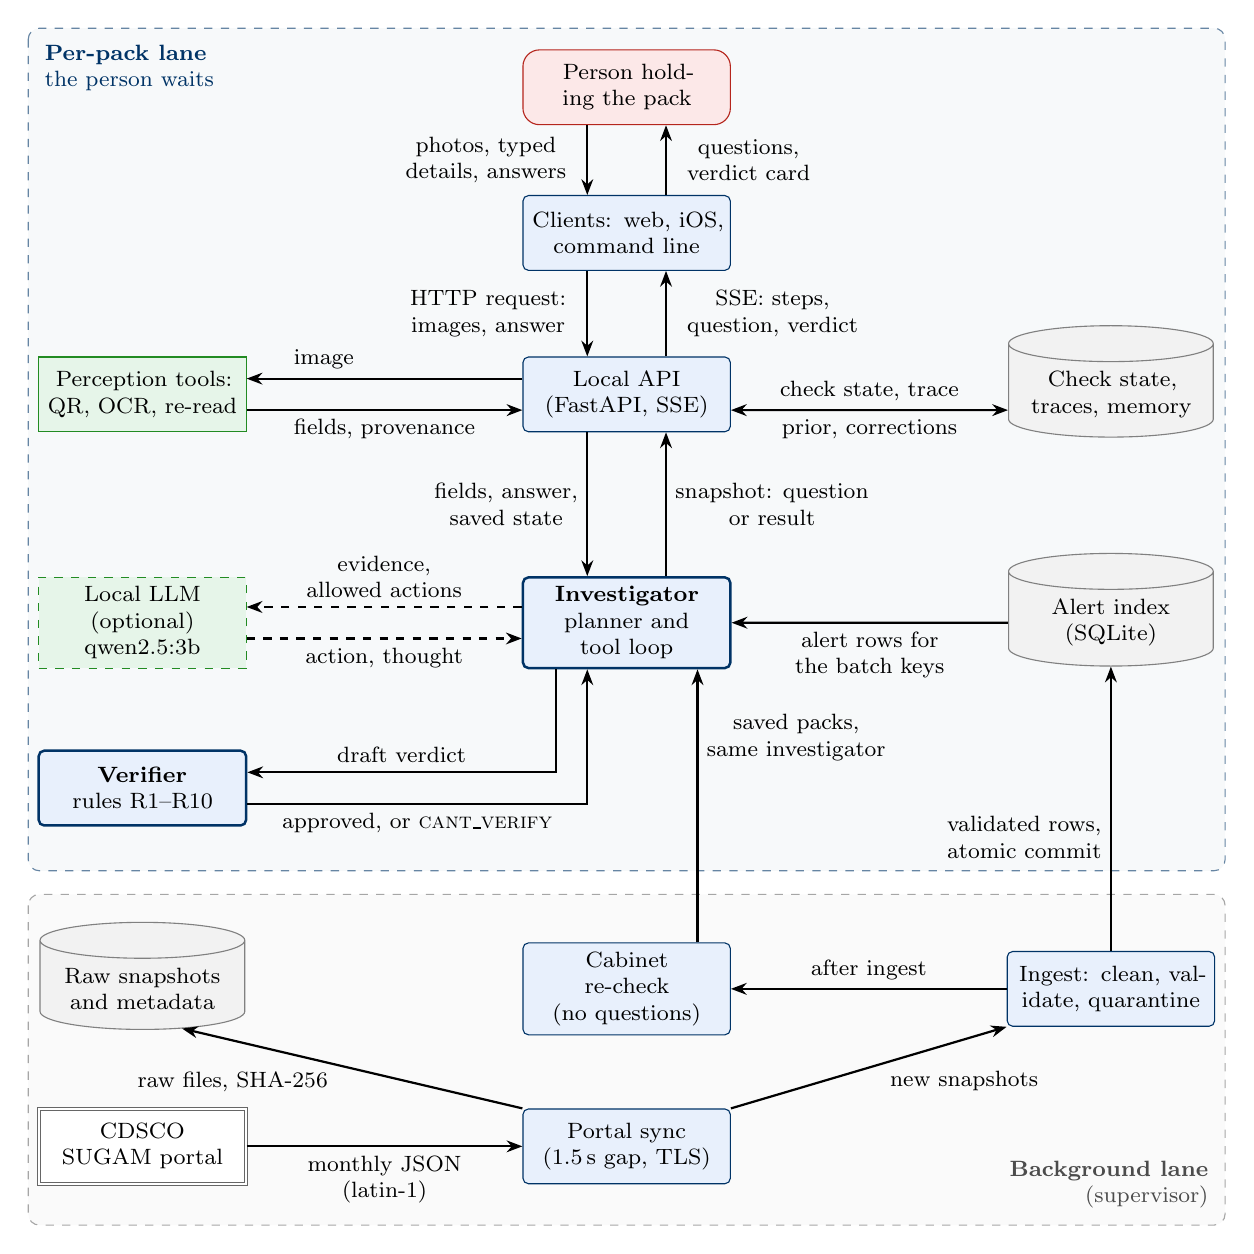
\begin{tikzpicture}[
  font=\footnotesize,
  box/.style={draw=bmsblue,fill=guidebg,rounded corners=2pt,minimum width=2.6cm,text width=2.4cm,minimum height=0.95cm,align=center},
  agent/.style={box,line width=0.9pt},
  tool/.style={draw=ForestGreen,fill=dobg,minimum width=2.6cm,text width=2.4cm,minimum height=0.95cm,align=center},
  opt/.style={tool,dashed},
  store/.style={draw=gray,fill=gray!10,cylinder,shape border rotate=90,aspect=0.18,minimum width=2.6cm,text width=2.3cm,minimum height=1.15cm,align=center},
  human/.style={draw=BrickRed,fill=dontbg,rounded corners=6pt,minimum width=2.6cm,text width=2.4cm,minimum height=0.95cm,align=center},
  ext/.style={draw=black!60,fill=white,minimum width=2.6cm,text width=2.4cm,minimum height=0.95cm,align=center,double},
  arr/.style={-{Stealth[length=2mm]},thick},
  lab/.style={font=\footnotesize,align=center,inner sep=3pt}]
% columns 1.3 / 7.45 / 13.6 ; rows below
\node[human] (person) at (7.45,0) {Person holding the pack};
\node[box]   (clients) at (7.45,-1.85) {Clients: web, iOS, command line};
\node[box]   (api) at (7.45,-3.9) {Local API (FastAPI, SSE)};
\node[tool]  (perc) at (1.3,-3.9) {Perception tools: QR, OCR, re-read};
\node[store] (state) at (13.6,-3.9) {Check state, traces, memory};
\node[agent] (inv) at (7.45,-6.8) {\textbf{Investigator} planner and tool loop};
\node[opt]   (llm) at (1.3,-6.8) {Local LLM (optional) qwen2.5:3b};
\node[store] (index) at (13.6,-6.8) {Alert index (SQLite)};
\node[agent] (ver) at (1.3,-8.9) {\textbf{Verifier} rules R1--R10};
\node[store] (raw) at (1.3,-11.45) {Raw snapshots and metadata};
\node[box]   (recheck) at (7.45,-11.45) {Cabinet\\re-check\\(no questions)};
\node[box]   (ingest) at (13.6,-11.45) {Ingest: clean, validate, quarantine};
\node[ext]   (portal) at (1.3,-13.45) {CDSCO SUGAM portal};
\node[box]   (sync) at (7.45,-13.45) {Portal sync\\(1.5\,s gap, TLS)};
% lanes
\begin{scope}[on background layer]
\draw[dashed,draw=bmsblue!60,fill=bmsblue!3,rounded corners=4pt] (-0.15,0.75) rectangle (15.05,-9.95);
\draw[dashed,draw=gray!70,fill=gray!4,rounded corners=4pt] (-0.15,-10.25) rectangle (15.05,-14.45);
\end{scope}
\node[anchor=north west,lab,align=left,text=bmsblue] at (-0.05,0.65) {\textbf{Per-pack lane}\\the person waits};
\node[anchor=south east,lab,align=right,text=black!70] at (14.95,-14.35) {\textbf{Background lane}\\(supervisor)};
% per-pack arrows
\draw[arr] ([xshift=-5mm]person.south) -- node[lab,left,xshift=-1.5mm]{photos, typed\\details, answers} ([xshift=-5mm]clients.north);
\draw[arr] ([xshift=5mm]clients.north) -- node[lab,right,xshift=1.5mm]{questions,\\verdict card} ([xshift=5mm]person.south);
\draw[arr] ([xshift=-5mm]clients.south) -- node[lab,left,xshift=-1.5mm]{HTTP request:\\images, answer} ([xshift=-5mm]api.north);
\draw[arr] ([xshift=5mm]api.north) -- node[lab,right,xshift=1.5mm]{SSE: steps,\\question, verdict} ([xshift=5mm]clients.south);
\draw[arr] ([yshift=2mm]api.west) -- node[lab,above,pos=0.72]{image} ([yshift=2mm]perc.east);
\draw[arr] ([yshift=-2mm]perc.east) -- node[lab,below]{fields, provenance} ([yshift=-2mm]api.west);
\draw[arr,{Stealth[length=2mm]}-{Stealth[length=2mm]}] ([yshift=-2mm]api.east) -- node[lab,above]{check state, trace} node[lab,below]{prior, corrections} ([yshift=-2mm]state.west);
\draw[arr] ([xshift=-5mm]api.south) -- node[lab,left]{fields, answer,\\saved state} ([xshift=-5mm]inv.north);
\draw[arr] ([xshift=5mm]inv.north) -- node[lab,right]{snapshot: question\\or result} ([xshift=5mm]api.south);
\draw[arr,dashed] ([yshift=2mm]inv.west) -- node[lab,above]{evidence,\\allowed actions} ([yshift=2mm]llm.east);
\draw[arr,dashed] ([yshift=-2mm]llm.east) -- node[lab,below]{action, thought} ([yshift=-2mm]inv.west);
\draw[arr] (index.west) -- node[lab,below]{alert rows for\\the batch keys} (inv.east);
\draw[arr] ([xshift=-9mm]inv.south) |- node[lab,above,pos=0.75]{draft verdict} ([yshift=2mm]ver.east);
\draw[arr] ([yshift=-2mm]ver.east) -| node[lab,below,pos=0.25]{approved, or \CANTV} ([xshift=-5mm]inv.south);
% background arrows
\draw[arr] (portal.east) -- node[lab,below]{monthly JSON\\(latin-1)} (sync.west);
\draw[arr] (sync.north west) -- node[lab,below left=-1pt,pos=0.55]{raw files, SHA-256} (raw.south east);
\draw[arr] (sync.north east) -- node[lab,below right=-1pt,pos=0.55]{new snapshots} (ingest.south west);
\draw[arr] (ingest.north) -- node[lab,left,pos=0.4]{validated rows,\\atomic commit} (index.south);
\draw[arr] (ingest.west) -- node[lab,above]{after ingest} (recheck.east);
\draw[arr] ([xshift=9mm]recheck.north) -- node[lab,right,pos=0.75]{saved packs,\\same investigator} ([xshift=9mm]inv.south);
\end{tikzpicture}
\caption{Architecture of StripCheck as built. Blue boxes are control components (bold: the agent and
its verifier), green boxes are tools, the dashed box is optional, cylinders are local stores and the
double box is the external data source.}
\label{fig:arch}
\end{figure}

Three decisions shape the figure. The agent is one bounded loop with an independent verifier,
because the question it answers (is this exact batch on a list?) has a fixed set of evidence steps
that a fixed loop can bound, test and trace. The language model sits beside the loop and never on
the path to the person: it chooses between two allowed actions at a branch point, and the rules take
over when it is slow, absent or invalid. The LangGraph graphs of the specification were replaced by
a custom loop whose whole state is one JSON document saved after every run, which keeps the pause
and resume behaviour with less code (decision D18).

\section{Component Description}
\label{sec:design-component-description}

This section describes every box of Figure~\ref{fig:arch}: its responsibility, inputs and outputs,
method and behaviour on failure.

\subsection{Clients and local API}

The web, iOS and command-line clients talk to one local FastAPI server. \texttt{POST /api/checks}
starts a check with one or two images or typed fields, and \texttt{POST /api/\allowbreak checks/<id>/\allowbreak resume}
continues it with an answer. Progress is streamed as server-sent events (\texttt{step},
\texttt{interrupt} for a question, \texttt{final} for the verdict and others) through a queue of 256
messages, and the work continues if the browser disconnects. The API passes the investigator only
the alert rows whose batch key matches the read or typed batch, together with the size and month
coverage of the whole index. A second answer to a running or changed check is refused with HTTP
409, and an unexpected error marks the check as failed. The server binds to \texttt{127.0.0.1};
phone access needs a pairing token.

\subsection{Perception tools}

Perception turns an image into pack fields, each with its source. A barcode reader (zxing-cpp,
then OpenCV) parses a QR or GS1 code; RapidOCR with PP-OCRv6-small models reads the printed lines on
the CPU~\cite{rapidai2021rapidocr,du2020ppocr}; one enhanced re-read is tried when no batch is found;
label-anchored patterns extract batch, product, brand, dates and maker. Each reader runs in a
separate process within a 60\,s deadline per photo. A failed read leaves the field empty, and the
investigator then asks the person to type the batch. If the QR and printed batches disagree, the
printed one is used without confirmed status; if two photos disagree, the person is asked.

\subsection{Planner}

The default planner is a fixed rule order (Section~\ref{sec:design-control-flow-and-agent-state}).
In hybrid mode the local model \texttt{qwen2.5:3b} under Ollama~\cite{ollama2026structured} is
consulted at two branch points: (b) after an empty exact search, choosing \texttt{search\_variants}
or \texttt{draft\_verdict}, and (c) when grading leaves a candidate that needs a person, choosing
\texttt{ask\_user} or \texttt{draft\_verdict}. It receives a JSON evidence object, the allowed
actions and the rule suggestion, and must return an allowed action and a one-sentence thought. On a
timeout (15\,s by default), a connection error, invalid JSON or an action outside the list, the rule
suggestion is used with the source \texttt{rules(fallback)}, and after a connection error the model
is skipped for 30\,s. A thought with a banned phrase is withheld. The model writes no text that the
person reads.

\subsection{Executor and tools}

The investigator runs each chosen action as a tool call and appends the observation to the history
of the check: \texttt{extract\_fields}, \texttt{search\_exact}, \texttt{search\_variants},
\texttt{grade}, \texttt{ask\_user} and \texttt{draft\_verdict} (signatures in
Chapter~\ref{ch:impl}). The tools are deterministic functions over local data. Inputs a tool cannot
use (no data loaded, a batch shorter than 2 or longer than 40 characters, an unreadable date) end the
run with a \CANTV{} draft and a stated reason instead of an exception.

\subsection{Retriever and relevance grader}

Retrieval is keyed on the normalised batch string, since batch codes carry no meaning that a
semantic search could use. \texttt{search\_exact} looks the key up; \texttt{search\_variants}
generates look-alike keys from a table of confusable characters (8 and B, 0 and O, 1 and I and
others) with at most two substitutions and 2{,}000 lookups, ordered by a noisy-channel score from
earlier confirmations~\cite{kernighan1990spelling,brill2000improved}. The variant search also runs
after an exact hit, so that a listed sibling batch is not missed. The grader treats each candidate as
a record-linkage decision~\cite{fellegi1969theory,christen2012survey}: a disagreeing product, brand
or maker rejects it (a batch collision); a substitution needs a character confirmation; a date one
digit off needs a date confirmation; missing product or maker evidence needs more printed details;
agreeing evidence accepts it. At most 20 candidates are graded.

\subsection{Reflector and human approval gate}

The verifier re-checks every draft against the stored state with ten hard rules (R1 to R10,
Table~\ref{tab:verifier}), independently of the drafting code. An alarm needs a corroborated
candidate, a confirmed batch and a citation; \NLISTED{} needs both searches, no pending candidate and
a statement of the lists loaded; every used field needs a source; no text may contain a banned
phrase. A failing draft becomes the \CANTV{} template with the rule ids. Only one draft is sent back
for revision: a model draft made before the variant search, which rule R4 returns once.

The human gate is \texttt{ask\_user}, with five question kinds: type the batch, confirm the batch,
confirm a character, confirm a printed date, or add printed details or a carton photo. An alarm
requires the batch to come from a QR code, from the person or from two agreeing photos, never from
OCR alone. The person types the characters at the look-alike positions instead of pressing a yes
button, because people tend to accept confirmations without
checking~\cite{parasuraman2010complacency,bucinca2021trust}. Every question offers ``Can't tell'',
and a declined question leads to \CANTV.

\subsection{Stores and memory}

The \emph{alert index} is a SQLite table of cleaned rows, each with its source URL, the SHA-256
digest of its snapshot and its row number. The \emph{check state} store keeps one JSON document per
check, written after every run so that a pending question survives a restart, and the same database
holds the cabinet of saved packs, notifications and confirmed character corrections; each check also
writes a JSON Lines trace. The \emph{raw snapshots} are the portal responses with their metadata.
Memory has two parts: the cabinet of saved packs, and a confusion prior of character pairs that
people confirmed on photographed packs. The prior reorders variants and chooses which characters to
ask about; it never removes a question.

\subsection{Background supervisor}

The portal sync fetches the newest three months by default (the history from January 2019 on
request), at least 1.5\,s apart, with TLS verification, three attempts and a 20\,s timeout, and
stores each raw response. Ingest reads the latin-1 JSON, validates the rows, quarantines rows with a
missing product, a placeholder batch or a date in the batch cell, and commits each snapshot in one
transaction; a snapshot whose digest is already stored is skipped, so imports are idempotent. The
cabinet re-check then runs the same investigator on every saved pack with questions disabled and
notifies the person of a new listing or a printed expiry within 30 days. When the portal is
unreachable the existing index stays in use.


\section{Selected Agentic Patterns and Justification}
\label{sec:design-selected-agentic-patterns-and-justification}

Table~\ref{tab:design-patterns} lists the patterns used, where each sits, why it was chosen and
which alternative was rejected. The common reason is the cost of an error: a false alarm on a
sibling batch harms a product that is not listed, and a confident \NLISTED{} can be read as an
assurance about the medicine. Every decision that reaches the person is therefore kept in testable
rules, and the model is used only where a later rule catches a wrong choice, in line with the advice
to prefer simple workflows when the steps are known~\cite{schluntz2024building}.

\begin{table}[!htbp]
\centering
\caption{Agentic patterns used in StripCheck and the alternatives rejected}
\label{tab:design-patterns}
\small\renewcommand{\_}{\textunderscore\allowbreak}
\begin{tabularx}{\linewidth}{@{}>{\raggedright\arraybackslash}p{2.6cm} >{\raggedright\arraybackslash}p{2.2cm} >{\raggedright\arraybackslash}X >{\raggedright\arraybackslash}p{2.9cm}@{}}
\toprule
\textbf{Pattern} & \textbf{Where} & \textbf{Reason} & \textbf{Alternative rejected} \\ \midrule
Bounded tool loop (plan, act, observe)~\cite{yao2023react} & Investigator & Each step is a logged tool call; the loop has a step cap and runs without a model & Free-form ReAct loop driven by the model \\
Model as advisor at branch points~\cite{kambhampati2024llmmodulo} & Planner (b), (c) & A 3B local model chooses only among allowed actions; rules check and replace its choice & Model plans every step \\
Corrective retrieval with a grader & Exact and variant search, grade & A misread batch is expected; an empty exact search triggers a bounded look-alike search, and grading removes collisions & Single exact lookup (the baseline of Chapter~\ref{ch:eval}) \\
Record linkage~\cite{fellegi1969theory} & Grader & A shared batch string is not identity; product, dates and maker must agree & Embedding similarity over alert text \\
External verifier (reflection)~\cite{huang2024cannot} & Verifier & Hard rules re-check the draft against stored state & Model self-critique~\cite{madaan2023selfrefine,shinn2023reflexion} \\
Human-in-the-loop interrupt & \texttt{ask\_user} & Only the person holding the pack can read the printed character & Yes/no confirm button; fully automatic alarm \\
Abstention~\cite{chow1970reject,geifman2017selective} & \CANTV{} & Weak evidence ends in an explicit ``more evidence is needed'' & Forced choice between alarm and \NLISTED \\
Supervisor with re-check & Background lane & Sequential sync, ingest, re-check with one investigator & Multi-agent conversation~\cite{wu2023autogen} \\
\bottomrule
\end{tabularx}
\end{table}

A model-driven ReAct loop was rejected because a 3B model on a laptop adds seconds per decision
and its choices cannot be bounded in advance; Chapter~\ref{ch:exp} later found that the hybrid
planner changed no verdict on the \ResN{} evaluation packs while its 95th-percentile latency was
about five times that of the rule planner. Model self-critique was rejected for the reason given
in Section~\ref{sec:lit-related-technical-work}: without external feedback it does not reliably
correct the model's reasoning.

\section{Control Flow and Agent State}
\label{sec:design-control-flow-and-agent-state}

Figure~\ref{fig:design-flow} shows the decision flow of one run of the investigator. A run starts
from the supplied fields, or resumes from the saved state with an answer. Every path ends in
\texttt{draft\_verdict} and the verifier, or in a question that pauses the check; there is no other
exit. The diamonds are the decision points, and the two branch points where the hybrid planner may
consult the model are marked (b) and (c).

\begin{figure}[!htbp]
\centering\setstretch{1}
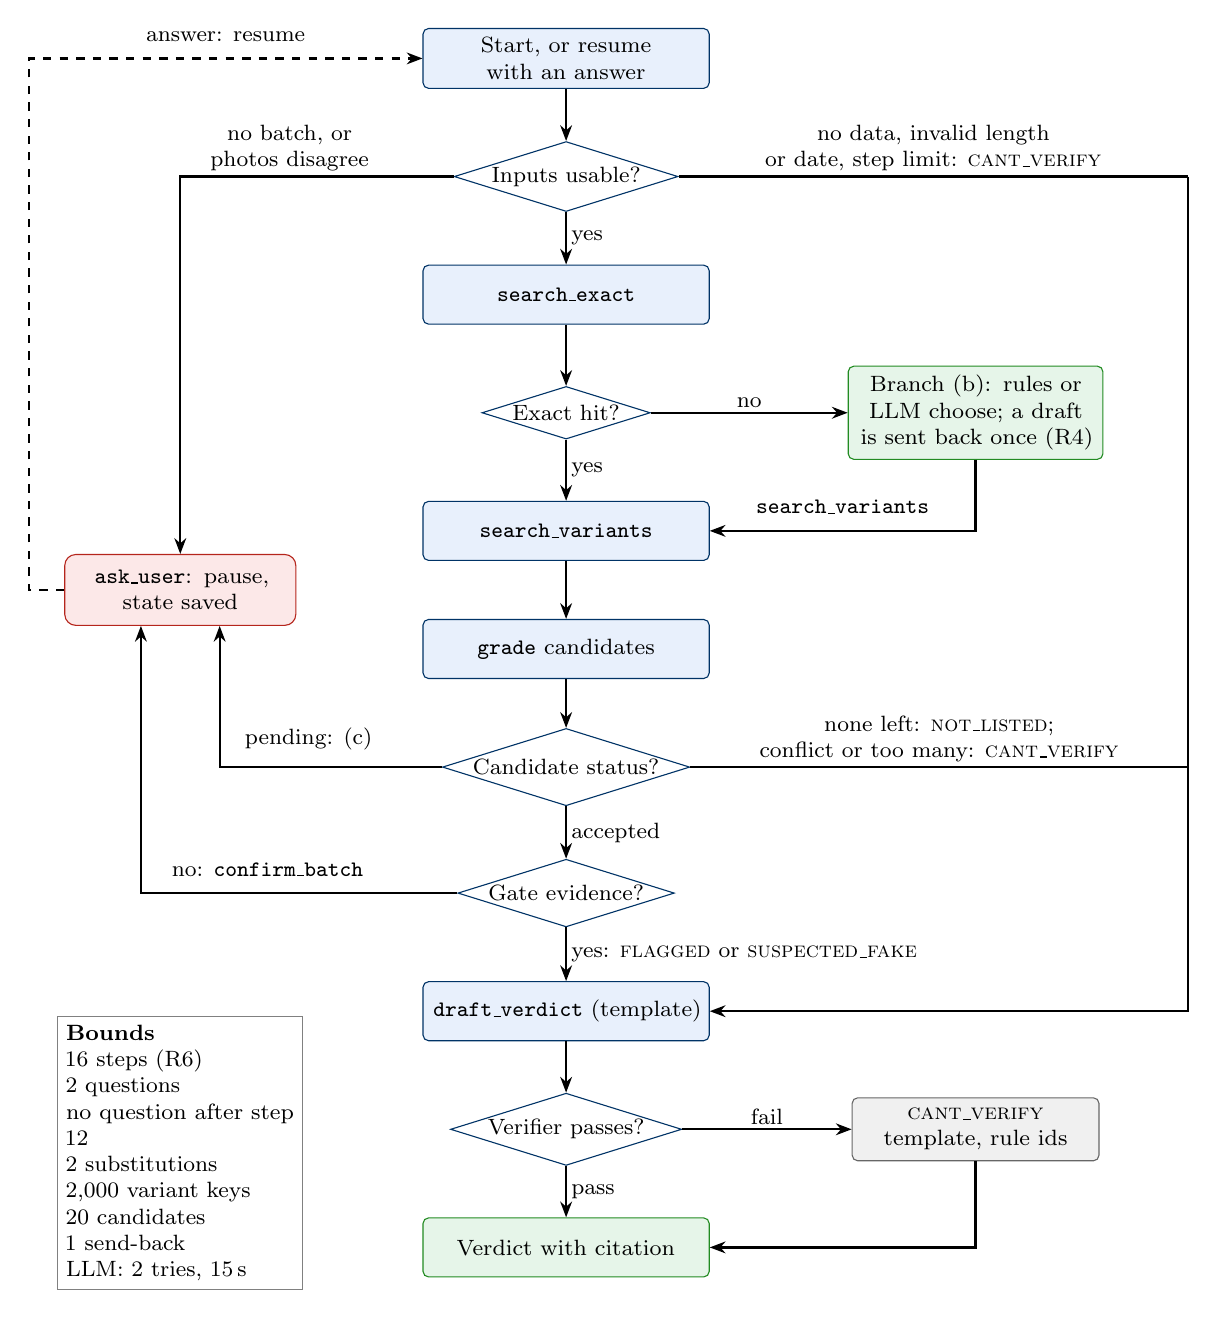
\begin{tikzpicture}[
  font=\footnotesize,
  stp/.style={draw=bmsblue,fill=guidebg,rounded corners=2pt,minimum width=3.6cm,text width=3.4cm,minimum height=0.75cm,align=center},
  dec/.style={draw=bmsblue,fill=white,diamond,aspect=3.2,inner sep=0.5pt,align=center},
  hum/.style={draw=BrickRed,fill=dontbg,rounded corners=4pt,text width=2.7cm,minimum height=0.9cm,align=center},
  side/.style={draw=ForestGreen,fill=dobg,rounded corners=2pt,text width=3.0cm,minimum height=0.8cm,align=center},
  bad/.style={draw=black!60,fill=gray!12,rounded corners=2pt,text width=2.9cm,minimum height=0.8cm,align=center},
  arr/.style={-{Stealth[length=2mm]},thick},
  lab/.style={font=\footnotesize,align=center,inner sep=1.5pt}]
\node[stp] (start) at (6.4,0) {Start, or resume with an answer};
\node[dec]  (d1) at (6.4,-1.5) {Inputs usable?};
\node[stp] (ex) at (6.4,-3.0) {\texttt{search\_exact}};
\node[dec]  (d2) at (6.4,-4.5) {Exact hit?};
\node[stp] (va) at (6.4,-6.0) {\texttt{search\_variants}};
\node[stp] (gr) at (6.4,-7.5) {\texttt{grade} candidates};
\node[dec]  (d3) at (6.4,-9.0) {Candidate status?};
\node[dec]  (d4) at (6.4,-10.6) {Gate evidence?};
\node[stp] (dr) at (6.4,-12.1) {\texttt{draft\_verdict} (template)};
\node[dec]  (d5) at (6.4,-13.6) {Verifier passes?};
\node[stp,fill=dobg,draw=ForestGreen] (out) at (6.4,-15.1) {Verdict with citation};
\node[hum]  (ask) at (1.5,-6.75) {\texttt{ask\_user}: pause, state saved};
\node[side] (pb) at (11.6,-4.5) {Branch (b): rules or LLM choose; a draft is sent back once (R4)};
\node[bad]  (cv) at (11.6,-13.6) {\CANTV{}\\template, rule ids};
\node[draw=black!50,fill=white,text width=2.9cm,align=left,inner sep=3pt] (bounds) at (1.5,-13.9)
  {\textbf{Bounds}\\16 steps (R6)\\2 questions\\no question after step 12\\2 substitutions\\2{,}000 variant keys\\20 candidates\\1 send-back\\LLM: 2 tries, 15\,s};
% spine
\draw[arr] (start) -- (d1);
\draw[arr] (d1) -- node[lab,right]{yes} (ex);
\draw[arr] (ex) -- (d2);
\draw[arr] (d2) -- node[lab,right]{yes} (va);
\draw[arr] (va) -- (gr);
\draw[arr] (gr) -- (d3);
\draw[arr] (d3) -- node[lab,right]{accepted} (d4);
\draw[arr] (d4) -- node[lab,right]{yes: \FLAGGED{} or \SFAKE} (dr);
\draw[arr] (dr) -- (d5);
\draw[arr] (d5) -- node[lab,right]{pass} (out);
% branch (b) and send-back
\draw[arr] (d2) -- node[lab,above]{no} (pb);
\draw[arr] (pb.south) |- node[lab,above,pos=0.75,yshift=1.5mm]{\texttt{search\_variants}} (va.east);
% questions
\draw[arr] (d1.west) -| node[lab,above,pos=0.3]{no batch, or\\photos disagree} (ask.north);
\draw[arr] (d3.west) -| node[lab,above,pos=0.3,yshift=1.5mm]{pending: (c)} ([xshift=5mm]ask.south);
\draw[arr] (d4.west) -| node[lab,above,pos=0.3,yshift=1.5mm]{no: \texttt{confirm\_batch}} ([xshift=-5mm]ask.south);
\draw[arr,dashed] (ask.west) -- ++(-0.45,0) |- node[lab,above,pos=0.75,yshift=1.5mm]{answer: resume} (start.west);
% abstention rail
\draw[thick] (d1.east) -- node[lab,above]{no data, invalid length\\or date, step limit: \CANTV} (14.3,-1.5);
\draw[arr] (14.3,-1.5) |- (dr.east);
\draw[thick] (d3.east) -- node[lab,above]{none left: \NLISTED;\\conflict or too many: \CANTV} (14.3,-9.0);
\draw[arr] (d5) -- node[lab,above]{fail} (cv);
\draw[arr] (cv.south) |- (out.east);
\end{tikzpicture}
\caption{Decision flow of one investigator run. Diamonds are decisions, (b) and (c) are the branch
points where the hybrid planner may consult the local model, red is the pause for a question, and
grey is the downgrade by the verifier. Every path reaches the verifier or a question.}
\label{fig:design-flow}
\end{figure}

A pending candidate leads to the matching question: \texttt{confirm\_char} for a substituted
character, \texttt{confirm\_field} for a date one digit off and \texttt{box\_photo} for missing
product or maker evidence. When no question may be asked, or the planner at (c) drafts, the reason
is drafted as \CANTV. After an answer the check resumes from the saved state, applies the answer to
the fields and runs the searches and the grader again. The state is one JSON document per check
(Table~\ref{tab:design-state} in Appendix~\ref{app:supp}), stored by the API after every run and loaded by the resume endpoint,
so a check can wait for an answer across a server restart.

Every loop in the design has an upper bound; Table~\ref{tab:design-bounds} in
Appendix~\ref{app:supp} lists the termination condition of each. The values are constants in \texttt{core/config.py} and the reader,
model and streaming modules, and settings read from the environment are clamped; the verifier
enforces the step and question limits again as rule R6, so a defect in the investigator cannot
produce an unbounded check that is still shown as a result.

\section{Data Flow}
\label{sec:design-data-flow}

This section follows one input end to end. The example is the recorded walkthrough of 8 November
2026 (\texttt{docs/trace/run1\_trace.jsonl}), run with the hybrid planner against a throwaway
database that holds one invented alert record (batch \texttt{LM2408B} for ``Lumera Tablets'' by
``Example Laboratories'', listed as NSQ in September 2026), so that no CDSCO row is copied. The pack
carries batch \texttt{LM2408B}, but the reader returned \texttt{LM24088}: the final B was read as 8.

Perception and the API pass the investigator the fields batch \texttt{LM24088}, product ``Lumera
Tablets'', manufacture 2024-08, expiry 2027-07 and the maker, each with provenance \texttt{ocr} and
batch evidence \texttt{ocr}. The exact search (step~2) returns 0 candidates. At branch point (b) the
model receives the read batch, the 0 exact hits and the allowed actions and returns
\texttt{search\_variants}, which finds one candidate, \texttt{LM2408B}, with the substitution 8 to B
at position~7 (step~3). Grading finds product, dates and maker in agreement and sets the status
\texttt{needs\_confirm\_char} (step~4). At branch point (c) the model returns \texttt{ask\_user}, the
check stores its state and pauses with a \texttt{confirm\_char} question (step~5). The person chooses
\texttt{LM2408B}; the batch is replaced, its evidence becomes \texttt{user\_confirmed}, and the pair
(8, B) is stored in the confusion prior (step~6). The searches and the grader run again on the
confirmed batch and accept the candidate (steps~7 to~9), and the \FLAGGED{} template with list,
month and source passes the verifier (step~10). Table~\ref{tab:app-trace1} in
Appendix~\ref{app:traces} lists the recorded steps.

A plain lookup would have answered \NLISTED{} at step 2. The model chose the same actions as the
rules at both branch points, and the check used 10 of its 16 steps and one of its two questions.

%---------------------------------------------------------------------
% Chapter 5: Agentic Concepts Demonstrated (template sections; see GUIDANCE.md)
% PLACEHOLDER: replace this comment with content.
%---------------------------------------------------------------------
\chapter{Agentic Concepts Demonstrated}
\label{ch:concepts}

\section{Concept Coverage Matrix}
\label{sec:concepts-concept-coverage-matrix}

\section{Evidence for Each Concept}
\label{sec:concepts-evidence-for-each-concept}

%---------------------------------------------------------------------
% Chapter 6: Implementation
% Sources: core/*.py, server/app.py, server/sse.py at HEAD 25fb3f8 (working copies of
% core/investigator.py, core/llm.py, core/templates.py, server/* are being edited by another
% workflow; facts here are from HEAD); versions from FACTS.md section 16; DB counts from a
% read-only query of data/stripcheck.db (FACTS.md section 25).
%---------------------------------------------------------------------
\chapter{Implementation}
\label{ch:impl}
\sloppy

This chapter describes how the design of Chapter~\ref{ch:design} was built: the software stack, the ingestion of the CDSCO portal data, the bounded agent loop, the tools, the prompt, the guardrails, the interfaces and the repository. With Appendix~\ref{app:run} it is meant to let another student rebuild and run the system.

\section{Technology Stack}
\label{sec:impl-technology-stack}

Table~\ref{tab:stack} lists the components with the versions installed on the Windows~11 laptop used for the evaluation (\texttt{pip list} and \texttt{ollama --version}, 12 November 2026). A check must finish with no network, no language model and no tracing server, and the project may not use paid services, so every component runs on the user's machine and the language model is optional.

\begin{table}[htbp]
\centering
\caption{Technology stack and installed versions}
\label{tab:stack}
\footnotesize
\begin{tabularx}{\linewidth}{@{}>{\raggedright\arraybackslash}p{2.6cm} >{\raggedright\arraybackslash}p{5.2cm} >{\raggedright\arraybackslash}X@{}}
\toprule
\textbf{Layer} & \textbf{Choice (version)} & \textbf{Reason} \\ \midrule
Language & Python 3.12.7 & One language for engine, ingest and evaluation \\
Agent engine & Own bounded loop, \texttt{core/investigator.py} & Small, testable, resumable (decision D18) \\
Storage & SQLite (standard library), WAL mode & One local file for alerts, checks, memory \\
API server & FastAPI 0.162.0, Uvicorn 0.54.0, Pydantic 2.14.1 & Streams steps and questions as server-sent events \\
Text reading & RapidOCR 3.10.0, PP-OCRv6-small on ONNX Runtime 1.31.1; Apple Vision on macOS & Local, CPU only, no download at run time \cite{rapidai2021rapidocr,du2020ppocr} \\
Barcodes & zxing-cpp 3.1.1; OpenCV headless 4.14.0.94 & GS1 payloads carry a check digit \\
Images & Pillow 13.0.0, pillow\_heif 1.8.1 & Validation, resizing, HEIC photos \\
Fuzzy matching & RapidFuzz 3.14.6 & Maker similarity in grading \\
Local LLM (optional) & Ollama 0.17.7, \texttt{qwen2.5:3b} & JSON-schema output from a local model \cite{ollama2026structured} \\
Tracing (optional) & OpenTelemetry SDK 1.45.1; Arize Phoenix 21.0.0 & Standard spans, viewed locally \cite{otel2026genai,arize2026openinference} \\
Clients & React 19.3.1, TypeScript 6.0.3, Vite 8.3.5; SwiftUI (iOS 17) & Step timeline, question cards, camera \\
Tests & pytest 9.1.1; Vitest 5.0.5 & Offline by default \\
\bottomrule
\end{tabularx}
\end{table}

The Review~2 design used LangGraph and Streamlit. LangGraph was replaced by a compact engine whose whole state is one JSON document, because the loop has few nodes and had to be resumable from any client (D18); Streamlit was replaced by FastAPI with a React client, because its rerun model fits poorly with a check that pauses for a question and streams each step (D2, D16).

\section{Data Preparation and Indexing}
\label{sec:impl-data-preparation-and-indexing}

\paragraph{Portal sync.} CDSCO's viewer for Not of Standard Quality (NSQ) and spurious drug alerts is embedded from the SUGAM portal, whose page script calls plain JSON endpoints \cite{cdsco2026portal}. \texttt{core/portal.py} calls \texttt{reportingYears} and \texttt{publicReportingMonths} to discover the published months of each tab, then fetches each month from \texttt{filteredNsqDrugTable} or \texttt{filteredSpuriousDrugTable}. A normal sync fetches the newest three months, which late state reports still change; \texttt{sync --full} fetches the history. Requests keep TLS verification on and obey the limits of Table~\ref{tab:design-bounds} (Appendix~\ref{app:supp}). The responses are Latin-1 (ISO-8859-1) and are decoded as such. The exact bytes are written atomically to \texttt{data/raw/portal/<kind>/YYYY-MM.json} (kind \texttt{nsq} or \texttt{spurious}) with a \texttt{.meta.json} file (URL, fetch time, SHA-256, row count, encoding), and a copy kept under its hash preserves older versions of a month. The database records 111 imported snapshots: 108 current months (93 NSQ, 15 spurious) and 3 superseded versions of NSQ months. An offline sync rebuilds the index from these files alone.

\paragraph{Parsing and validation.} \texttt{core/ingest.py} maps the portal fields (\texttt{str\_product\_name}, \texttt{str\_brand\_name}, \texttt{str\_batch\_no}, \texttt{str\_manufactured\_by}, \texttt{dt\_manufacturing\_date}, \texttt{dt\_expiry\_date}, \texttt{str\_nsq\_result}, \texttt{str\_reported\_by\_lab\_or\_state} and others) to one row shape. Descriptive text is repaired only when it shows reversible UTF-8/Latin-1 damage, and batch and date cells are never repaired. A brand in brackets after the product name moves to the brand field, a GS1 prefix ``(10)'' is removed from the batch, and a cell that lists several batches is split into one row per batch. Dates are parsed to year and month, the maker is separated from the marketer, and the entry type (NSQ, spurious, misbranded or adulterated) is derived from the tab, the spurious flag and the result text. Rows that can still be matched keep warning flags; rows that cannot be matched reliably go to a quarantine table with their reasons and stay visible in the interface. No language model repairs rows. Of the rows fetched, 75 are in quarantine; Table~\ref{tab:ingest} in Appendix~\ref{app:run} gives the outcomes by reason.


\paragraph{Idempotent import and indexing.} Each cleaned row gets a hash of its raw cells, list month, list kind and batch key. A snapshot whose SHA-256 and cleaning version were already imported adds no rows; a changed snapshot of the same month supersedes the old source and marks vanished rows as removed. The table holds 6{,}953 rows, of which \ResAlertCount{} are active and 30 removed, and each import runs in one transaction. The match key is the batch in upper case with every character other than A--Z and 0--9 removed, under a partial SQLite index on active rows. A check fetches only the exact key and up to 2{,}000 look-alike keys with \texttt{IN} queries in chunks of 400. Embeddings and a vector store do not fit this task: a batch number is an identifier, and semantic similarity would retrieve exactly the near neighbours that must not be confused. Retrieval therefore uses exact keys and an explicit table of look-alike characters, and the uncertainty of the reading becomes a question.

\section{Core Agent Loop}
\label{sec:impl-core-agent-loop}

Algorithm~\ref{alg:loop} is one call of \texttt{investigate()} in \texttt{core/investigator.py}. The server calls it when a check starts and after every answer; between calls the state is stored as a JSON document in SQLite.

\begin{algorithm}[htbp]
\caption{Bounded investigation of one check (one call)}
\label{alg:loop}
\footnotesize
\begin{algorithmic}[1]
\Require fields $f$, alert rows $A$, stored state $\sigma$ or none, answer $a$ or none; $S{=}16$ steps, $Q{=}2$ questions, $K{=}20$ candidates
\If{$\sigma$ is none} $\sigma \gets$ new state; \textsc{Log}(\texttt{extract\_fields}) \EndIf
\If{$\sigma.\mathit{pending}$}
  \If{$a$ is none} \Return $\sigma$ \Comment{still waiting} \EndIf
  \State \textsc{ApplyAnswer}$(\sigma, f, a)$; $\sigma.\mathit{asks} \gets \sigma.\mathit{asks}+1$ \Comment{malformed answer: re-ask}
\EndIf
\State $\mathit{canAsk} \gets \sigma.\mathit{asks} < Q \wedge |\sigma.H| < S-4$
\If{no alert data \textbf{or} batch length outside 2--40 \textbf{or} unparseable date \textbf{or} $|\sigma.H| \ge S-3$} $\ell \gets$ \CANTV
\ElsIf{no batch \textbf{or} two photos disagree} \textbf{if} $\mathit{canAsk}$ \textbf{return} \textsc{Ask}(\texttt{type\_batch}) \textbf{else} $\ell \gets$ \CANTV
\Else
  \State $E \gets \textsc{SearchExact}(A, \mathit{key}(f))$
  \If{$E = \emptyset$ \textbf{and} \textsc{Decide}$(\{\texttt{search\_variants}, \texttt{draft\_verdict}\}) = \texttt{draft\_verdict}$} \Comment{branch (b)}
    \State \textsc{Log}(verifier send-back, rule R4) \Comment{at most once}
  \EndIf
  \State $V \gets \textsc{SearchVariants}(A, \mathit{key}(f))$ \Comment{$\le 2$ substitutions, $\le 2000$ keys}
  \State $C \gets \textsc{Grade}(\text{first } K \text{ of } E \cup V, f)$
  \If{a date conflict in $C$ \textbf{or} more than $K$ candidates} $\ell \gets$ \CANTV
  \ElsIf{a candidate in $C$ needs a person}
    \If{$\mathit{canAsk} \wedge \textsc{Decide}(\{\texttt{ask\_user}, \texttt{draft\_verdict}\}) = \texttt{ask\_user}$} \Return \textsc{Ask}(kind) \Comment{branch (c)} \EndIf
    \State $\ell \gets$ \CANTV
  \ElsIf{a candidate $c \in C$ is accepted}
    \If{batch evidence is not QR, typed, confirmed or two agreeing reads}
      \State \textbf{if} $\mathit{canAsk}$ \textbf{return} \textsc{Ask}(\texttt{confirm\_batch}) \textbf{else} $\ell \gets$ \CANTV
    \Else{} $\ell \gets$ \SFAKE{} if $c$ is spurious, else \FLAGGED \EndIf
  \Else{} $\ell \gets$ \NLISTED \EndIf
\EndIf
\State \Return \textsc{Verify}(\textsc{Render}$(\ell, f, c)$, $\sigma$) \Comment{template text; a failing draft becomes \CANTV}
\end{algorithmic}
\end{algorithm}

\textsc{ApplyAnswer} validates the answer against the pending question (for example one letter or digit per requested position) and returns an error without counting it when the answer is malformed. A new question is allowed only while fewer than two have been asked and the history has fewer than 12 steps, so the steps after the last answer still fit within 16. The variant search runs after an exact hit too, so a listed sibling batch one character away is not missed. \textsc{Decide} returns the rule suggestion in rule mode and whenever the model fails. \textsc{Log} drops steps once 16 are recorded, and verifier rule R6 rejects any draft whose history exceeds 16 steps or two questions, so the loop stays bounded even if a later change breaks a guard.

\section{Tools and Function Definitions}
\label{sec:impl-tools-and-function-definitions}

The agent calls the tools named in Algorithm~\ref{alg:loop}; Table~\ref{tab:tools} in Appendix~\ref{app:supp} lists each with its input, output, bounds and failure behaviour. None is mocked: every tool runs on the real index or the real image. The demonstration packs and evaluation cartons are synthetic images, and their records are marked synthetic and excluded from real checks.

\paragraph{OCR pipeline on Windows and macOS.} \texttt{read\_pack} validates the upload (at most 15\,MB and 24 million pixels), shrinks it so no side exceeds 2{,}400 pixels and gives the whole read a 60\,s deadline. Barcodes are tried first (zxing-cpp, then Apple Vision on macOS, then OpenCV) in a process killed at its deadline; GS1 application identifiers 10, 11 and 17 give the batch and dates. Text is read by Apple Vision on macOS and, on Windows, by Tesseract if installed or otherwise by a persistent RapidOCR worker that loads the pinned PP-OCRv6-small models once (D23) and never downloads models. When no batch is found, the image is read once more after grey-scaling, auto-contrast and sharpening. Label-anchored patterns (``B.No.'', ``Batch No'', ``Lot'', ``BN'') then find the batch, dates and maker, and every value keeps its source (\texttt{qr} or \texttt{ocr}).

\paragraph{Matching and noisy-channel ranking.} \texttt{search\_variants} generates every key reachable from the read key by one or two substitutions from a table of characters that OCR confuses on printed codes (for example \texttt{B}/\texttt{8}/\texttt{3}, \texttt{0}/\texttt{O}/\texttt{D}/\texttt{Q}/\texttt{C}, \texttt{1}/\texttt{I}/\texttt{L}/\texttt{7}/\texttt{T}, \texttt{5}/\texttt{S}, \texttt{2}/\texttt{Z}). Hits are ordered by the number of substitutions, then by the channel score of Equation~\eqref{eq:channel}, then by row id:
\begin{equation}
s(v \mid r) = \sum_{i \in S} \log \frac{n_{r_i v_i} + \alpha}{n_{r_i r_i} + \alpha}, \qquad \alpha = 1,
\label{eq:channel}
\end{equation}
where $r$ is the read key, $v$ the variant, $S$ the substituted positions and $n_{ab}$ the number of times a read character $a$ was confirmed as printed $b$. This follows the noisy-channel view of spelling and OCR correction \cite{kernighan1990spelling,brill2000improved,kolak2002ocr}. With no stored counts the score is zero. The score never changes a character by itself: a variant hit always needs the person's confirmation, and the same counts order the positions asked in a batch confirmation, most doubtful first (D25).

\paragraph{Grading.} \texttt{grade} compares each candidate with the pack field by field. Product and brand evidence is the share of the entry's name tokens found on the pack, ignoring dosage words (match from 0.8, partial from 0.5); dates are compared by year and month; the maker matches at a RapidFuzz token-set ratio of at least 85. A product or brand mismatch rejects the candidate as a collision. An exact batch with an unknown product or a disagreeing maker needs more evidence, a one-digit date difference becomes a date question and a larger one is a conflict that ends in \CANTV{}. A variant batch needs a character confirmation. An NSQ entry is accepted when the dates or the maker agree, a spurious entry when the dates agree or the entry lists none, because the listed maker of a spurious entry is often ``under investigation''.

\section{Prompt Design}
\label{sec:impl-prompt-design}

The language model is used only by \texttt{plan\_decision} in \texttt{core/llm.py}, at the two branch points. Each request to Ollama's \texttt{/api/chat} carries a fixed system message, a user message that wraps a task sentence, the evidence object, the allowed actions and the rule suggestion as JSON, and a JSON schema that requires a \texttt{thought} of at most 240 characters and an \texttt{action} from the allowed list, with temperature~0 and at most 256 reply tokens. Appendix~\ref{app:prompts} gives the verbatim strings (Listings~\ref{lst:app-system} and~\ref{lst:app-planner}).


The system message and the JSON wrapping keep pack and alert text inside data fields, because OCR text from a photo is untrusted input that could contain instructions. The schema, passed as Ollama's \texttt{format} \cite{ollama2026structured}, restricts the action to the allowed list, so the model can reorder evidence gathering but cannot invent a tool or a verdict. The evidence object holds only derived facts (read batch and source, hit counts or candidate status, questions left, learned confusions). Temperature~0 makes the choice repeatable. The thought is capped at 240 characters, stripped of non-printable characters and replaced by a fixed notice if it contains a banned phrase. No prompt produces user-facing text.

\section{Guardrails and Loop Bounds}
\label{sec:impl-guardrails-and-loop-bounds}

Every bound and timeout is listed with its termination behaviour in Table~\ref{tab:design-bounds} (Appendix~\ref{app:supp}). The values are constants in \texttt{core/config.py}, \texttt{investigator.py}, \texttt{llm.py}, \texttt{pack\_tools.py} and \texttt{server/sse.py}; settings read from the environment are clamped to the ranges shown there.


\paragraph{Verifier.} \texttt{core/verifier.py} re-checks every draft against the stored state, independently of the drafting code, with the rules of Table~\ref{tab:verifier}. On any violation the draft is replaced by the \CANTV{} template and the rule identifiers are stored with the check; when only the batch gate (R2) fails, the text names the batch and month that would match and asks the person to have a pharmacist check the batch.

\begin{table}[htbp]
\centering
\caption{Verifier rules as implemented}
\label{tab:verifier}
\footnotesize
\begin{tabularx}{\linewidth}{@{}l >{\raggedright\arraybackslash}X@{}}
\toprule
\textbf{Rule} & \textbf{Condition checked on the draft and the stored state} \\ \midrule
R1 & The label is one of the four verdicts \\
R2 & An alarm needs an accepted candidate with an exact or confirmed batch, batch evidence from QR, two agreeing reads or the person, a product match (or a partial match with dates and maker), no field mismatch, and equal batch keys \\
R3 & \SFAKE{} only for a spurious entry; \FLAGGED{} only for NSQ, misbranded or adulterated entries \\
R4 & \NLISTED{} needs a grounded batch, both searches run, no pending or accepted candidate, loaded data, no truncation \\
R5 & An alarm cites the entry with a source URL or SHA-256; no text contains a banned phrase \\
R6 & At most 16 steps and 2 questions \\
R7 & Outside \CANTV, no candidate has an unresolved date conflict \\
R8 & Outside \CANTV, every field used has a grounded source (person, OCR, QR, enhanced OCR, carton) \\
R9 & \NLISTED{} states the lists loaded and the latest list month \\
R10 & The verdict language is a reviewed one (English) \\
\bottomrule
\end{tabularx}
\end{table}

\paragraph{Templates.} All user-facing text comes from \texttt{core/templates.py}. The headlines are fixed: ``This batch is on an alert list'' (\FLAGGED), ``This batch is listed as purported spurious'' (\SFAKE), ``No matching alert found'' (\NLISTED) and ``More evidence is needed'' (\CANTV). An alarm names the list month, the failed test and the reporting laboratory and ends with ``Show this pack to your pharmacist. Do not stop any prescribed medicine without medical advice.'' A not-listed result states the lists loaded and the latest month, and adds that it does not certify the medicine because CDSCO tests only sampled batches. A case-insensitive pattern blocks the banned words of the safety policy (with Hindi equivalents) in every template and in text copied from alert rows, and the verifier and the tests enforce it. Only the listed batch is flagged, never a brand, and the web client never shows \NLISTED{} in green.

\section{User Interface}
\label{sec:impl-user-interface}

\paragraph{API.} \texttt{server/app.py} serves a FastAPI application on 127.0.0.1:8000. \texttt{POST /api/checks} accepts one or two photos or typed fields, and \texttt{POST /api/checks/<id>/resume} accepts an answer; both stream server-sent events (\texttt{fields}, \texttt{strip}, \texttt{candidates}, \texttt{step}, \texttt{interrupt}, \texttt{snapshot}, \texttt{final}, \texttt{report}, \texttt{done}, \texttt{error}), and the work continues if the browser disconnects. A check that is running, or that changed since the client loaded it, refuses a second answer. Further endpoints serve the alert library, quarantine, the cabinet, the per-check trace and phone pairing; with \texttt{--lan} every request needs a pairing token.

\paragraph{Clients.} Figure~\ref{fig:ui-check} in Appendix~\ref{app:supp} shows the start of a check in the React web client. While a check runs, the screen shows a step timeline (action, source, summary) and a batch strip whose character cells change from read to uncertain or confirmed; a question appears as a card with one input per requested character or a choice between the read and the listed batch, and the verdict card shows the template text with its citation. A SwiftUI client for iOS uses the same API with the camera; it was built and tested in the simulator in CI and not on a physical device. \texttt{cli.py} runs sync, ingest, checks, diagnostics and the evaluation.

\section{Repository Structure}
\label{sec:impl-repository-structure}

The repository has \texttt{cli.py} at the top, the engine in \texttt{core/} (Table~\ref{tab:modules} in Appendix~\ref{app:run}), the API in \texttt{server/}, the clients in \texttt{web/} and \texttt{ios/}, tests in \texttt{tests/}, decisions and results in \texttt{docs/}, evaluation outputs in \texttt{runs/} and the paper and this report in \texttt{paper/}. The \texttt{data/} folder (snapshots, database, uploads, traces) is excluded from version control, because the alert data stay local.

\fussy

%---------------------------------------------------------------------
% Chapter 7: Observability and Evaluation
% Numbers: \res{...} macros from ../generated/results.tex (run 2, seed 7); the few hand-typed
% values (reasoning p95, Phoenix span times, error counts) are sourced in FACTS.md sections 12 and 23.
%---------------------------------------------------------------------
\chapter{Observability and Evaluation}
\label{ch:eval}

This chapter describes how a check is made visible while it runs and how the agent was measured
against a simpler lookup. All numbers come from our own runs. Evaluation numbers come from
\texttt{paper/generated/results.tex}, written by \texttt{cli.py eval}; the few values typed by hand
(the reasoning 95th percentile, the Phoenix span times and the error counts) are taken from
\texttt{docs/results/eval\_seed7.md} and \texttt{docs/trace/} and listed in \texttt{FACTS.md}. The reported run is the second run on the evaluation seed; the first run and the
code changes between the two are disclosed in Chapter~\ref{ch:exp}.

\section{Tracing and Monitoring}
\label{sec:eval-tracing-and-monitoring}

\begingroup\setlength{\emergencystretch}{3em}
\paragraph{JSONL step log.} Every check writes one JSON-lines file, named
\texttt{data/\allowbreak traces/\allowbreak <thread\_id>.jsonl}, which the API serves at \texttt{GET /api/traces/<id>}.
Each line carries the UTC time, the check identifier and the event name. Step events add the step
number, the action, the planner source (\texttt{rules}, \texttt{llm}, \texttt{rules(fallback)},
\texttt{rules(verifier)} or \texttt{user}), a one-line summary and the duration in milliseconds, and,
where present, the planner's thought, the learned prior and the verifier result (event list in
Section~\ref{sec:concepts-observability}). The schema has fields for the model name and token
counts that the current code does not fill, so token usage is not reported; the model name and the
duration of each model call are recorded in the OpenTelemetry span described next. Cost is zero by
construction, because the only model is a local one. A failure in the tracer is swallowed, so
writing a trace can never fail a check. The same events stream to the client over server-sent
events and drive its live step timeline.\par\endgroup

\paragraph{OpenTelemetry and Phoenix.} When \texttt{STRIPCHECK\_TRACING=1} is set, the same check
is exported as OpenTelemetry spans to a local Arize Phoenix server (version 21.0.0) using the
OpenInference conventions~\cite{otel2026genai,arize2026openinference}. A 0.25\,s TCP probe, cached
for 15\,s, skips span creation when Phoenix is not running, and the exporter has a 3\,s timeout.
Each check becomes one trace: a root \texttt{check} span (\textsc{agent}), a
\texttt{planner:~<action>} span per step (\textsc{chain}) with its \textsc{tool} span, a
\texttt{planner\_llm} span (\textsc{llm}) at each model consultation, a \texttt{verifier} span
(\textsc{guardrail}), and a \texttt{check.resume} span for the half after an answer.

Figure~\ref{fig:phoenix-trace} shows the span tree of the misread walkthrough of
Section~\ref{sec:design-data-flow} (25 spans). In the exported spans (\texttt{docs/trace/phoenix\_spans\_run1.json}) the two
\texttt{planner\_llm} spans took 4.60\,s and 3.89\,s of the 8.49\,s root span, and every tool span
took under a millisecond, so the model calls account for almost all of the time. Phoenix shows
these durations truncated to one decimal (4.5\,s, 3.8\,s and 8.4\,s), and the 8.8\,s in its header is
the trace latency that Phoenix measures for the whole trace, including the resumed half. The root
span's input and output are shown in Figure~\ref{fig:app-phoenix-io} of Appendix~\ref{app:traces}.
With Ollama unreachable, the same check finished in about 2\,s with \texttt{rules(fallback)} at both
branch points and the same \FLAGGED{} result (\texttt{docs/trace/README.md}), which is the behaviour
the fallback is designed for.

\begin{figure}[htbp]
\centering
\begin{tikzpicture}
\node[anchor=south west,inner sep=0] (img) at (0,0)
  {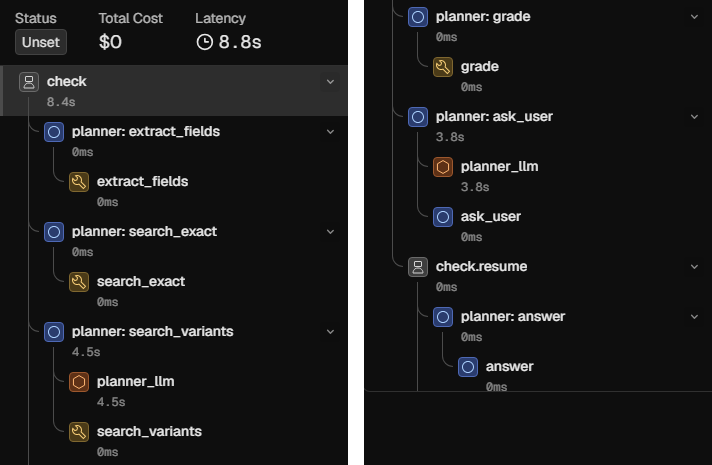
\includegraphics[width=\linewidth]{fig_phoenix_tree.png}};
\begin{scope}[x={(img.south east)},y={(img.north west)},
  callout/.style={circle,fill=BrickRed,text=white,font=\bfseries\footnotesize,inner sep=1.2pt,minimum size=13pt}]
  \node[callout] at (0.405,0.914) {1};  % trace latency and cost
  \node[callout] at (0.160,0.824) {2};  % root check span (agent)
  \node[callout] at (0.285,0.166) {3};  % planner_llm before search_variants
  \node[callout] at (0.805,0.630) {4};  % planner_llm before ask_user
  \node[callout] at (0.775,0.424) {5};  % check.resume
\end{scope}
\end{tikzpicture}
\caption{Span tree of the Review~3 misread walkthrough in Phoenix (synthetic pack, hybrid planner),
cropped and split into two columns; the right column continues the left one. (1)~trace latency
8.8\,s and cost \$0 (local model); (2)~root \texttt{check} span of kind \textsc{agent} (8.49\,s,
shown truncated as 8.4\,s); (3)~branch point after the empty exact search, where the model chose
\texttt{search\_variants} (4.60\,s); (4)~branch point after grading, where the model chose
\texttt{ask\_user} (3.89\,s); (5)~the resumed half of the check under the same root.}
\label{fig:phoenix-trace}
\end{figure}

\paragraph{Monitoring.} The evaluation harness counts steps by planner source (model or fallback),
and \texttt{cli.py doctor} reports the database counts, the installed readers and whether Ollama
and Phoenix are reachable.

\section{Evaluation Dataset}
\label{sec:eval-evaluation-dataset}

Eleven authored diagnostic scenarios check behaviour in the test suite and are not used as an
accuracy measure. The evaluation uses the golden set generated by \texttt{cli.py props --eval}, which renders
\res{ResN} cartons from real alert rows of the local index of \res{ResAlertCount} alerts, and every
image carries the banner ``DEMO PROP - NOT A MEDICINE''. No team member labels the packs by hand:
the generator writes the truth label and the printed fields of each pack to a manifest when it
renders the carton, so labels are correct by construction. Clean, glare, QR, misread and spurious
packs carry a listed batch (40 packs); not-listed controls carry an invented batch, collisions a
listed batch number on a different product and maker, and siblings an unlisted batch one look-alike
character from a listed one (20 packs). Table~\ref{tab:eval-mix} in Appendix~\ref{app:supp} gives
the count and truth label of each scenario. Two seeds
of the generator give two disjoint sets of packs. Seed~1 is the development set, on which the
thresholds were tuned, and seed~\res{ResSeed} is the evaluation set reported here. Misread and
sibling packs print the misread string on the carton, so the OCR error is simulated, and the oracle
user answers from the batch the pack was meant to carry (decision D24). Perception is shared by all
arms and runs once per image: the reader (RapidOCR PP-OCRv6-small) returned the rendered batch on
\res{ResOCRBatchExact} images of seed~\res{ResSeed}, at a median of \res{ResOCRMedian}\,s per image.

\section{Metrics and Evaluation Rubric}
\label{sec:eval-metrics-and-evaluation-rubric}

Let $P$ be the packs whose truth is \FLAGGED{} or \SFAKE{}, $N$ the packs whose truth is \NLISTED{},
$A=\{\FLAGGED,\SFAKE\}$ the alarm labels and $\hat{y}_i$ the label an arm returns for pack $i$. The
metrics are defined as in \texttt{core/evaluate.py}:
\begin{align*}
\text{hit recall} &= \frac{|\{i\in P:\hat{y}_i\in A\}|}{|P|}, &
\text{type accuracy} &= \frac{|\{i\in P:\hat{y}_i=y_i\}|}{|\{i\in P:\hat{y}_i\in A\}|},\\[2pt]
\text{false-alarm rate} &= \frac{|\{i\in N:\hat{y}_i\in A\}|}{|N|}, &
\text{abstention rate} &= \frac{|\{i:\hat{y}_i=\CANTV\}|}{n}.
\end{align*}
The false-alarm rate is also reported on the collision and sibling packs alone. Overall accuracy is
the share of all packs whose label equals the truth. Questions per pack and steps per pack are
averages over all packs. Latency per pack is the shared perception time plus the arm's own reasoning
time; we report the median, the mean and the 95th percentile (linear interpolation). A safety
violation is a banned phrase in the headline, explanation or advice, an unknown label, or an alarm
without a citation, and the required count is zero.

Rates carry 95\% Wilson score intervals~\cite{wilson1927probable,brown2001interval}, which stay
inside $[0,1]$ and behave well at $k=0$ and $k=n$, where most of our cells lie. Paired comparisons
on the same packs use the exact two-sided McNemar test~\cite{mcnemar1947note,dietterich1998approximate}
on per-pack correctness, $p=\min\bigl(1,\,2\sum_{i=0}^{\min(b,c)}\binom{b+c}{i}2^{-(b+c)}\bigr)$,
where $b$ counts packs only the agent gets right and $c$ packs only the baseline gets right. With at
most eight packs per scenario, per-scenario results are given as counts.

No language model judges the output: the verdict is one of four discrete labels and the truth is
fixed by the manifest, so each pack is scored by exact comparison.

\section{Baselines}
\label{sec:eval-baselines}

Arm~A, the baseline, is a lookup script that does what a person can do with the CDSCO list viewer:
it takes the batch from the QR code or OCR, normalises it, looks it up exactly in the index and
reports any hit as an alarm (\SFAKE{} for a spurious entry, \FLAGGED{} otherwise). It uses the same
perception output, the same index of \res{ResAlertCount} alerts and the same verdict templates as
the agent, so the arms differ only in the reasoning between the read batch and the verdict. Arm~B is the agent with the rule planner and arm~C the agent with the
hybrid planner, which consults \texttt{qwen2.5:3b} through Ollama at the two branch points
(temperature~0). Each arm runs under two human-in-the-loop policies: an \emph{oracle} user who
answers every question truthfully from the manifest, and \emph{none}, where every question is
skipped. The second policy acts as an ablation of the human loop.

\section{Results}
\label{sec:eval-results}

Table~\ref{tab:eval-results} gives the headline metrics for the three arms under both policies.

\begin{table}[htbp]
\centering
\caption[Headline metrics on the evaluation set (seed~7, run~2)]{Headline metrics on the evaluation set (seed~7, $n=60$, run~2). Rates as value ($k/n$) with
the Wilson 95\% interval below. Source: \texttt{paper/generated/results.tex}.}
\label{tab:eval-results}
\footnotesize
\setlength{\tabcolsep}{4pt}
\renewcommand{\arraystretch}{1.12}
\begin{tabularx}{\linewidth}{@{}>{\raggedright\arraybackslash}X ccc@{}}
\toprule
\textbf{Metric} & \textbf{Baseline (lookup)} & \textbf{Agent (rules)} & \textbf{Agent (hybrid)} \\
\midrule
\multicolumn{4}{@{}l}{\textit{HITL = oracle (a person answers every question)}} \\
Hit recall & \res{ResBaseOracleHitRecall} (\res{ResBaseOracleHitRecallK}) & \res{ResRulesOracleHitRecall} (\res{ResRulesOracleHitRecallK}) & \res{ResHybridOracleHitRecall} (\res{ResHybridOracleHitRecallK}) \\
 & \res{ResBaseOracleHitRecallCI} & \res{ResRulesOracleHitRecallCI} & \res{ResHybridOracleHitRecallCI} \\
Hit recall, clean and QR & \res{ResBaseOracleHitRecallCleanQR} (\res{ResBaseOracleHitRecallCleanQRK}) & \res{ResRulesOracleHitRecallCleanQR} (\res{ResRulesOracleHitRecallCleanQRK}) & \res{ResHybridOracleHitRecallCleanQR} (\res{ResHybridOracleHitRecallCleanQRK}) \\
Type accuracy & \res{ResBaseOracleTypeAcc} (\res{ResBaseOracleTypeAccK}) & \res{ResRulesOracleTypeAcc} (\res{ResRulesOracleTypeAccK}) & \res{ResHybridOracleTypeAcc} (\res{ResHybridOracleTypeAccK}) \\
False-alarm rate, all not listed & \res{ResBaseOracleFAR} (\res{ResBaseOracleFARK}) & \res{ResRulesOracleFAR} (\res{ResRulesOracleFARK}) & \res{ResHybridOracleFAR} (\res{ResHybridOracleFARK}) \\
 & \res{ResBaseOracleFARCI} & \res{ResRulesOracleFARCI} & \res{ResHybridOracleFARCI} \\
False-alarm rate, collisions & \res{ResBaseOracleFARCollision} (\res{ResBaseOracleFARCollisionK}) & \res{ResRulesOracleFARCollision} (\res{ResRulesOracleFARCollisionK}) & \res{ResHybridOracleFARCollision} (\res{ResHybridOracleFARCollisionK}) \\
False-alarm rate, siblings & \res{ResBaseOracleFARSibling} (\res{ResBaseOracleFARSiblingK}) & \res{ResRulesOracleFARSibling} (\res{ResRulesOracleFARSiblingK}) & \res{ResHybridOracleFARSibling} (\res{ResHybridOracleFARSiblingK}) \\
Abstention rate & \res{ResBaseOracleAbstain} (\res{ResBaseOracleAbstainK}) & \res{ResRulesOracleAbstain} (\res{ResRulesOracleAbstainK}) & \res{ResHybridOracleAbstain} (\res{ResHybridOracleAbstainK}) \\
Overall accuracy & \res{ResBaseOracleAccuracy} (\res{ResBaseOracleAccuracyK}) & \res{ResRulesOracleAccuracy} (\res{ResRulesOracleAccuracyK}) & \res{ResHybridOracleAccuracy} (\res{ResHybridOracleAccuracyK}) \\
 & \res{ResBaseOracleAccuracyCI} & \res{ResRulesOracleAccuracyCI} & \res{ResHybridOracleAccuracyCI} \\
Questions / steps per pack & \res{ResBaseOracleQuestions} / \res{ResBaseOracleSteps} & \res{ResRulesOracleQuestions} / \res{ResRulesOracleSteps} & \res{ResHybridOracleQuestions} / \res{ResHybridOracleSteps} \\
Latency median / mean / p95 (s) & \res{ResBaseOracleLatMedian} / \res{ResBaseOracleLatMean} / \res{ResBaseOracleLatPNinetyFive} & \res{ResRulesOracleLatMedian} / \res{ResRulesOracleLatMean} / \res{ResRulesOracleLatPNinetyFive} & \res{ResHybridOracleLatMedian} / \res{ResHybridOracleLatMean} / \res{ResHybridOracleLatPNinetyFive} \\
LLM steps / fallback steps & \res{ResBaseOracleLLMSteps} / \res{ResBaseOracleFallbackSteps} & \res{ResRulesOracleLLMSteps} / \res{ResRulesOracleFallbackSteps} & \res{ResHybridOracleLLMSteps} / \res{ResHybridOracleFallbackSteps} \\
Safety violations & \res{ResBaseOracleSafety} & \res{ResRulesOracleSafety} & \res{ResHybridOracleSafety} \\
\midrule
\multicolumn{4}{@{}l}{\textit{HITL = none (every question skipped)}} \\
Hit recall & \res{ResBaseSkipHitRecall} (\res{ResBaseSkipHitRecallK}) & \res{ResRulesSkipHitRecall} (\res{ResRulesSkipHitRecallK}) & \res{ResHybridSkipHitRecall} (\res{ResHybridSkipHitRecallK}) \\
 & \res{ResBaseSkipHitRecallCI} & \res{ResRulesSkipHitRecallCI} & \res{ResHybridSkipHitRecallCI} \\
Hit recall, clean and QR & \res{ResBaseSkipHitRecallCleanQR} (\res{ResBaseSkipHitRecallCleanQRK}) & \res{ResRulesSkipHitRecallCleanQR} (\res{ResRulesSkipHitRecallCleanQRK}) & \res{ResHybridSkipHitRecallCleanQR} (\res{ResHybridSkipHitRecallCleanQRK}) \\
False-alarm rate, all not listed & \res{ResBaseSkipFAR} (\res{ResBaseSkipFARK}) & \res{ResRulesSkipFAR} (\res{ResRulesSkipFARK}) & \res{ResHybridSkipFAR} (\res{ResHybridSkipFARK}) \\
Abstention rate & \res{ResBaseSkipAbstain} (\res{ResBaseSkipAbstainK}) & \res{ResRulesSkipAbstain} (\res{ResRulesSkipAbstainK}) & \res{ResHybridSkipAbstain} (\res{ResHybridSkipAbstainK}) \\
Overall accuracy & \res{ResBaseSkipAccuracy} (\res{ResBaseSkipAccuracyK}) & \res{ResRulesSkipAccuracy} (\res{ResRulesSkipAccuracyK}) & \res{ResHybridSkipAccuracy} (\res{ResHybridSkipAccuracyK}) \\
Safety violations & \res{ResBaseSkipSafety} & \res{ResRulesSkipSafety} & \res{ResHybridSkipSafety} \\
\bottomrule
\end{tabularx}
\end{table}


With the oracle user both agent arms raised an alarm on all \res{ResRulesOracleHitRecallK} listed
packs and on none of the \res{ResRulesOracleFARK} not-listed packs. The lookup missed the eight
misread packs and raised an alarm on all eight collisions and all four siblings, so its false-alarm
rate on not-listed packs was \res{ResBaseOracleFAR} (\res{ResBaseOracleFARK}). On the clean, QR and
spurious packs the two approaches agree. Figure~\ref{fig:eval-scenarios} breaks the result down by
scenario and shows that the baseline fails exactly where a batch number alone is misleading.

\begin{figure}[htbp]
\centering
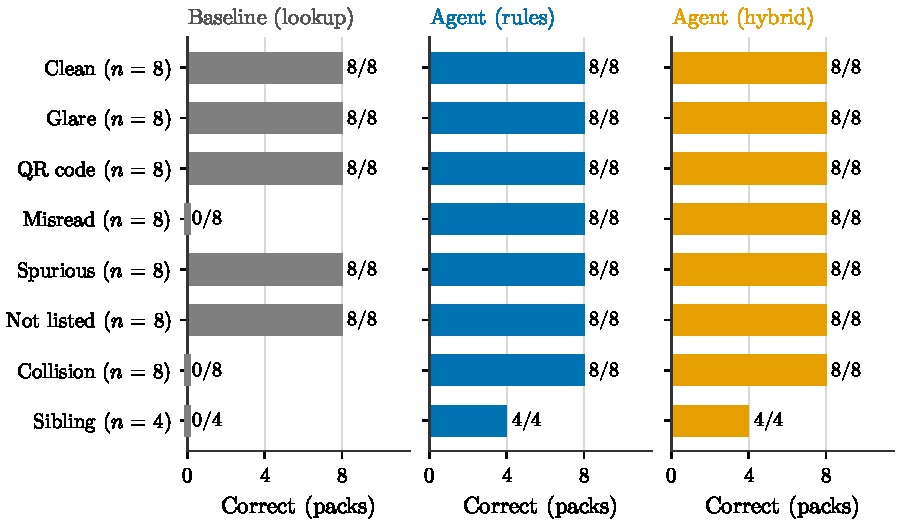
\includegraphics{fig_scenarios_seed7.pdf}
\caption{Correct verdicts per scenario on seed~7 with a person answering ($n=8$ per scenario, 4 for
siblings). ``Not listed'' denotes the not-listed control packs. The baseline fails on the misread,
collision and sibling packs.}
\label{fig:eval-scenarios}
\end{figure}

The agent's advantage depends on the person. When every question is skipped
(Figure~\ref{fig:eval-hitl} in Appendix~\ref{app:supp}), hit recall falls to \res{ResRulesSkipHitRecall}
(\res{ResRulesSkipHitRecallK}) and the agent abstains on \res{ResRulesSkipAbstainK} packs, which is
lower accuracy than the lookup (\res{ResRulesSkipAccuracyK} against \res{ResBaseSkipAccuracyK}). The
false-alarm rate stays at \res{ResRulesSkipFAR}, because rule R2 never turns an unconfirmed
machine read into an alarm. The packs it still gets right without answers are the QR packs, whose
batch is confirmed by the code, and the collision and not-listed control packs, which end in
\NLISTED{} without a question.

Figure~\ref{fig:eval-latency} (Appendix~\ref{app:supp}) gives the cost. Perception dominates every arm: the median end-to-end
time was \res{ResBaseOracleLatMedian}\,s for the lookup and \res{ResRulesOracleLatMedian}\,s for the
rule agent, whose reasoning took a median of \res{ResRulesOracleReasonMedian}\,s (95th percentile
0.103\,s). The hybrid planner had \res{ResHybridOracleFallbackSteps} fallbacks to rules. Its median rose only to
\res{ResHybridOracleLatMedian}\,s, because the model is consulted only at branch points
(\res{ResHybridOracleLLMSteps} times over \res{ResN} packs), but each model call
takes seconds on the laptop, so its 95th percentile was \res{ResHybridOracleLatPNinetyFive}\,s.
No arm produced a safety violation.

\section{Error Analysis}
\label{sec:eval-error-analysis}

Table~\ref{tab:eval-errors} groups every incorrect verdict of run~2 on seed~7, taken from the
per-pack listing in \texttt{docs/results/eval\_seed7.md}. Examples are schematic, because the packs
carry batch strings from CDSCO rows. With the oracle user the two agent arms
made no error, so the table lists the baseline's 20 errors and the agent's 36 abstentions when
questions are skipped. The seven alarms the agent missed in run~1, before the fixes, are analysed
in Section~\ref{sec:exp-results}.

\begin{table}[htbp]
\centering
\caption{Incorrect verdicts on seed~7 (run~2) grouped by cause, with one example per group}
\label{tab:eval-errors}
\small
\begin{tabularx}{\linewidth}{@{}>{\raggedright\arraybackslash}p{0.21\linewidth} c
  >{\raggedright\arraybackslash}X >{\raggedright\arraybackslash}p{0.25\linewidth}@{}}
\toprule
\textbf{Arm and cause} & \textbf{Count} & \textbf{Example} & \textbf{What addresses it} \\
\midrule
Baseline: misread batch not found & 8 & A listed \texttt{Z} printed as \texttt{2} (schematic:
listed \texttt{AZ1234}, carton \texttt{A21234}); lookup returns \NLISTED & Confusion-aware variant search with a person
confirming the character (agent) \\
Baseline: collision raised as alarm & 8 & Listed batch number on a different product and maker;
lookup returns \FLAGGED & Grading of product, dates and maker before any alarm (agent) \\
Baseline: sibling raised as alarm & 4 & Carton reads a listed batch one look-alike character
away from the unlisted batch the pack carries (schematic: \texttt{AB1703} read, \texttt{AB1708}
carried); lookup returns \FLAGGED & Batch confirmation by the person before an
alarm (agent) \\
Agent, no answers: batch gate & 28 & Clean, glare, spurious and sibling packs whose
\texttt{confirm\_batch} question was skipped end in \CANTV & A QR code or a second photo as
independent evidence; otherwise only the person \\
Agent, no answers: character unconfirmed & 8 & Misread packs whose \texttt{confirm\_char} question
was skipped end in \CANTV & Only the person holding the pack \\
\bottomrule
\end{tabularx}
\end{table}

The baseline's errors are structural. A lookup cannot recover a batch that the reader got wrong, and
it cannot tell whether a listed batch number belongs to this product, so collisions and siblings
become false alarms. The test set over-represents these traps by design, so this false-alarm rate
is not an estimate of the rate in use (Section~\ref{sec:lim-limitations}).
The agent's 36 abstentions are the designed behaviour of the batch gate; their cost is recall
without a human, which only stronger independent evidence (a QR code on more packs, or a second
agreeing read) can reduce. These results show that the reasoning behaves as designed on rendered traps; they do not
measure accuracy on photographs of real strips (Chapter~\ref{ch:lim}).

%---------------------------------------------------------------------
% Chapter 8: Experimentation (template sections; see GUIDANCE.md)
% PLACEHOLDER: replace this comment with content.
%---------------------------------------------------------------------
\chapter{Experimentation}
\label{ch:exp}

\section{Hypothesis}
\label{sec:exp-hypothesis}

\section{Experimental Setup}
\label{sec:exp-experimental-setup}

\section{Results}
\label{sec:exp-results}

\section{Discussion and Decision}
\label{sec:exp-discussion-and-decision}

%---------------------------------------------------------------------
% Chapter 9: Limitations, Ethics and Safety
% Sources: FACTS.md sections 1, 4, 5, 9, 11, 12, 14, 22; paper/sections/08_limitations.tex;
% core/investigator.py, core/verifier.py, core/llm.py, core/templates.py, core/config.py at HEAD 25fb3f8.
% Numbers: \res{} macros (paper/generated/results.tex, run 2), \RunOne* (paper/run1_results.tex),
% stats macros (paper/generated/stats.tex), seed 1 from paper/report/data/eval_seed1.md.
%---------------------------------------------------------------------
\chapter{Limitations, Ethics and Safety}
\label{ch:lim}

This chapter states what the results do not show, how StripCheck can fail and who could be harmed by a wrong result.

\section{Limitations}
\label{sec:lim-limitations}

\subsection{Data}
A \NLISTED{} verdict is only as good as the lists behind it. CDSCO tests only sampled batches, so a batch absent from the lists can still be substandard, and every \NLISTED{} result says so (verifier rule R9). The lists also describe the past: in the design-phase snapshot the median time from manufacture to the alert month is \LagMedian{} months (interquartile range \LagQOne{} to \LagQThree{}), so a batch that is substandard today may appear on a list many months later.

The index covers the portal from \FirstMonth{} to \LastMonth{}; alerts published only as PDF files before 2019 are absent. A brand name is present in only \BrandPresentPct\% of NSQ rows, so grading relies on the generic product text, the manufacturer and the printed dates, and the collisions and look-alike neighbours among batch keys (Section~\ref{sec:intro-motivation-and-why-agentic-ai}) keep the confirmation questions necessary.

\subsection{Method}
The confusion-aware search only explores the look-alike pairs in the fixed \texttt{CONFUSABLE} table of \texttt{core/textutils.py}, with at most two substitutions and at most 2,000 variant keys per search. A misread outside the table, or one with three changed characters, is not recovered, and the check then ends in \NLISTED{} for a listed batch. The vision-language second reader in the design was not built (decision D7), so independent batch evidence comes only from a QR code, a second photo that reads the same batch, or the person holding the pack.

The agent's recall depends on the person answering its questions: with every question skipped its hit recall falls to \res{ResRulesSkipHitRecallK}, below the lookup's \res{ResBaseSkipHitRecallK} (Chapter~\ref{ch:eval}), so the system is useful only to a person who can read the printed batch. The 3-billion-parameter model's thoughts are not always exact: in the walkthrough one thought swapped the read and listed batch (Appendix~\ref{app:traces}), an error that stays in the trace because the action comes from an allowed list.

A person who confirms the wrong character teaches the local confusion prior a wrong pair; the prior never skips a question, which limits the damage, but no mechanism yet removes a wrong entry.

\subsection{Evaluation}
Every pack in the evaluation and in the demonstrations is synthetic, rendered from real alert rows; no photographs of real medicine strips were taken. Rendered text flatters OCR (60 of 60 batches read correctly on seed~7), and embossed foil, curved bottles, glare and poor light are untested, so the results say nothing yet about accuracy on real strips. The OCR errors of the misread and sibling scenarios are simulated on the carton (decision D24). The oracle user answers every question correctly, while a real person may misread the pack or skip the question.

The test set is small. Each scenario holds at most eight packs, so the Wilson 95\% interval for a collision false-alarm rate of 0/8 still reaches \res{ResRulesOracleFARCollisionCI}, and small differences between arms are noise. Three defects found in run~1 were fixed before run~2 (decision D25), so run~2 is no longer a held-out test and its scores are an optimistic estimate; the development seed, from the same generator, gave the same agent results (Chapter~\ref{ch:exp}). The test set over-represents traps by design: 12 of the 60 packs are collisions or siblings. How often such traps occur on a real shelf was not measured, so neither the lookup's false-alarm rate in use nor the positive predictive value of an alarm can be read from these results. Latency was measured on one laptop, and the model's device was recorded only for the seed-1 run (GPU), so the latency of the two seeds is not compared. No usability study, no ablation of the confirmation gate (rule R-B of the design) and no comparison of language models were run. No LLM judge is used: every verdict is scored against the label stored in the evaluation manifest.

\section{Failure Modes and Guardrails}
\label{sec:lim-failure-modes-and-guardrails}

Table~\ref{tab:lim-risks} in Appendix~\ref{app:supp} pairs ten failure modes with the guardrail that addresses each and the place where it is enforced. The main ones are the variant search with a character question for a confident misread, record-linkage grading for a batch collision, the allowed-action list, timeout and rule fallback for a failing model, JSON-only prompts for instructions hidden in pack text, the banned-phrase rule for reassuring wording, and the step, question and candidate limits for unbounded loops. All guardrails are deterministic code; none depends on the language model behaving well.

Several were exercised in recorded runs. The model fallback with Ollama stopped is reported in Section~\ref{sec:eval-tracing-and-monitoring}. With every question skipped, the agent raised no false alarm on the 20 \NLISTED{} packs and abstained on \res{ResRulesSkipAbstainK} packs (Appendix~\ref{app:traces}); on the clean scenario a \FLAGGED{} draft built on an OCR-only batch returned \CANTV{} with rules R2 and R8 recorded. Safety violations were \res{ResRulesOracleSafety} in every arm and condition.

Some failure modes have no complete guardrail. A person who confirms the wrong character produces a wrong but confirmed batch, and the system cannot detect this. A listed batch that the reader misreads outside the look-alike table ends in \NLISTED{}, which is why that verdict never appears in green and always says that it does not certify the medicine.

\section{Ethical and Responsible-Use Considerations}
\label{sec:lim-ethical-and-responsible-use-considerations}

\paragraph{Who could be harmed.} A false alarm could worry a patient and, in the worst case, lead them to stop a prescribed medicine, so every alarm carries the fixed advice to show the pack to a pharmacist and not to stop a prescribed medicine without medical advice, and cites the CDSCO record. A false alarm could also harm a manufacturer, so only the listed batch is flagged, never a brand. A missed alarm could reassure a person wrongly, so the \NLISTED{} wording says that the result does not certify the medicine. Reassuring words and instructions to stop a medicine are blocked by the verifier, and the language model writes no user-facing text.

\paragraph{Advisory status.} StripCheck is a student project and not a CDSCO service, and the interface says so. Its output is advisory and directs the person to a pharmacist. No listed result is shown on a batch read only by OCR: the batch must come from a QR code, from two agreeing photos or from the person (rule R2).

\paragraph{Privacy.} Photos, checks, the confusion memory and the alert data stay on the user's computer; no account is created, and the check path makes no network call. Phone access needs a pairing token, and anyone holding the tunnel link can use the demonstration while it runs, so the tunnel is meant only for short supervised sessions.

\paragraph{Fairness and access.} The system serves people who can photograph a pack and read English; regional-language templates are withheld until a native speaker reviews them (rule R10). The OCR models were not evaluated on the range of print styles found on Indian packs, and errors could fall more heavily on some manufacturers' packaging.

\paragraph{Data.} The alert data from the CDSCO portal~\cite{cdsco2026portal} is fetched politely (requests at least 1.5~s apart, TLS verification on), kept locally and cited on every alarm, and this report publishes only derived statistics. The use of AI coding assistants is described in Appendix~\ref{app:contrib}.

%---------------------------------------------------------------------
% Chapter 10: Conclusion and Future Work (template sections; see GUIDANCE.md)
% Numbers: \res{...} from ../generated/results.tex (run 2, seed 7), stats macros from
% ../generated/stats.tex, run-1 macros from ../run1_results.tex. No new results here.
%---------------------------------------------------------------------
\chapter{Conclusion and Future Work}
\label{ch:concl}

\section{Conclusion}
\label{sec:concl-conclusion}

This report addressed a gap between CDSCO's batch-level quality alerts and the medicine pack in a
person's hand. The design follows from two properties measured in the alert data: batch numbers
collide across unrelated products, and listed batches have confusable siblings from the same
manufacturer. A batch match alone therefore cannot justify an alarm, and a confident OCR reading
cannot justify a miss. StripCheck answers with a bounded agent that searches for likely misreads,
grades every candidate field by field, asks the person to read the characters in doubt before any
alarm, and lets a rule-based verifier downgrade any draft the evidence does not support. Every loop
is bounded and every model call has a fallback, so the whole check runs offline on a laptop.

On the evaluation set of \res{ResN} rendered packs, with a person answering the questions, the
agent removed the baseline's collision and sibling false alarms (\res{ResRulesOracleFARCollisionK}
and \res{ResRulesOracleFARSiblingK} against \res{ResBaseOracleFARCollisionK} and
\res{ResBaseOracleFARSiblingK}) and raised hit recall from \res{ResBaseOracleHitRecall} to
\res{ResRulesOracleHitRecall} at \res{ResRulesOracleQuestions} questions per pack. Without answers
it abstained on \res{ResRulesSkipAbstainK} packs and still raised no false alarm, so the questions
carry the recall. These numbers come from the second run on the same packs. The first run reached
the same decision with a hit recall of \RunOneRulesOracleHitRecall; three general defects found in
it were fixed before the second run, so the reported figures are optimistic and the set is no
longer a blind test. Table~\ref{tab:concl-objectives} revisits each objective of
Section~\ref{sec:intro-objectives}.

\begin{table}[htbp]
\centering
\caption{Objectives from Section~\ref{sec:intro-objectives} and the outcome for each}
\label{tab:concl-objectives}
\small
\begin{tabularx}{\textwidth}{@{}c X l@{}}
\toprule
No. & Outcome & Status \\
\midrule
1 & The ingest stores every portal snapshot with its hash and quarantines invalid rows; the index
holds \res{ResAlertCount} alerts from \FirstMonth{} to \LastMonth{}. The snapshot analysis measured
\CollisionKeys{} collision keys, \SiblingKeys{} same-manufacturer siblings and a median lag of
\LagMedian{} months from manufacture to alert. & Met \\
2 & The rule agent completed every evaluation check offline, at \res{ResRulesOracleSteps} steps per
pack and a median reasoning time of \res{ResRulesOracleReasonMedian}\,s, within the bounds of 16
steps and two questions. & Met \\
3 & The verifier rejects any alarm draft without confirmed batch evidence; the false-alarm rate on not-listed packs
was \res{ResRulesOracleFARK} with answers and \res{ResRulesSkipFARK} without, and no arm produced
a safety violation. & Met \\
4 & Every check writes a step-level trace with action, source and rationale; the export to a local
Phoenix server was demonstrated on a recorded walkthrough. & Met \\
5 & Under the decision rule the agent is adopted when the person answers
(\res{ResRulesOracleDecision}) and not adopted when nobody answers
(\res{ResRulesSkipDecision}). The result is optimistic, as stated above. & Met, with caveat \\
6 & The hybrid planner gave the same label on all \res{ResN} packs and met the latency condition on
the median, so the rule held; the rule planner was kept as default because the hybrid's
95th-percentile time was \res{ResHybridOracleLatPNinetyFive}\,s against
\res{ResRulesOracleLatPNinetyFive}\,s. & Met \\
\bottomrule
\end{tabularx}
\end{table}

On these packs the gain over the lookup came from the deterministic parts of the agent, since
the optional LLM planner changed no verdict. How much each part contributes was not measured,
because the planned ablation of the confirmation gate was not run. The system stays advisory throughout. A \NLISTED{} result states which
lists were loaded and that it does not certify the medicine, and every alarm directs the person to
a pharmacist.

\section{Future Work}
\label{sec:concl-future-work}

Each item below follows from a limitation stated in Chapter~\ref{ch:lim}.
\begin{enumerate}[itemsep=2pt]
\item \emph{Real packs and a held-out set.} All evaluation packs are rendered images, and the
evaluation seed was run twice with fixes in between. The next step is a fresh seed together with
photos of real strips, bottles and cartons under varied light, which would measure OCR errors
instead of simulating them.
\item \emph{A study with people.} The oracle answers every question correctly, while real users may
misread a character or skip the question, and the recall depends on those answers. A usability
study should measure how often people answer, how accurately, and whether they understand that
\NLISTED{} does not certify a medicine.
\item \emph{Wider list coverage.} The index starts in January 2019. An adapter for the earlier PDF
months and for state-level alert feeds would extend the coverage that every \NLISTED{} result
depends on.
\item \emph{Regional languages.} Verdicts are shown in English only, because no Hindi or Kannada
template has been reviewed by native speakers. Reviewed templates, together with voice prompts,
would serve users who do not read English.
\item \emph{An independent second reader and a pharmacy workflow.} A local vision-language reader
was planned as independent batch evidence but not built. Adding it, and a pharmacist workflow that
checks a whole delivery against the lists, would move the check earlier, before a listed batch
reaches a patient.
\end{enumerate}


%=====================================================================
%  REFERENCES
%=====================================================================
% Use only keys that exist in ../references.bib (IEEE style via IEEEtran.bst).
\bibliographystyle{IEEEtran}
\bibliography{../references}

%=====================================================================
%  APPENDICES
%=====================================================================
\appendix
% Appendix A: Team Contribution.
% Source: paper/sections/10_contributions.tex (rows confirmed by the team lead on 2026-11-08); FACTS.md section 15.
% No percentage shares are given because none were confirmed by the team.
\chapter{Team Contribution}
\label{app:contrib}

Table~\ref{tab:app-contrib} records who owned each part of StripCheck and who led each project review. The table reproduces the mapping confirmed by the team lead for the project paper. Ownership means that the member designed the part, wrote or directed its code and tests, and answered for it at the reviews. The four members reviewed one another's modules, and every member can explain the whole system, from the portal sync to the verdict template. The code was written with AI coding assistants under the team's direction, and every module was reviewed and tested by the team.

\begin{table}[H]
\centering
\caption{Contribution of team members}
\label{tab:app-contrib}
\small
\renewcommand{\arraystretch}{1.2}
\begin{tabularx}{\linewidth}{@{}l >{\raggedright\arraybackslash}p{0.2\linewidth} >{\raggedright\arraybackslash}X >{\raggedright\arraybackslash}p{0.17\linewidth}@{}}
\toprule
\textbf{USN} & \textbf{Name} & \textbf{Components owned} & \textbf{Led review} \\
\midrule
\USNa & \NameA & Investigator and verifier, planner, tracing, interfaces & R3 trace walkthrough \\
\USNb & \NameB & Portal sync, ingest, alert index, matching, cabinet and memory & Data plan \\
\USNc & \NameC\ (lead) & Pack-reading tools, demonstration packs, integration, data analysis, report & R1, demonstrations \\
\USNd & \NameD & Evaluation harness, test sets, A/B experiment, results & R4 results \\
\bottomrule
\end{tabularx}
\end{table}

\begin{sloppypar}The modules behind each row are as follows. The investigator and verifier are \texttt{core/investigator.py} and \texttt{core/verifier.py}, the planner's model calls are in \texttt{core/llm.py}, tracing is \texttt{core/tracing.py}, and the interfaces are \texttt{server/}, \texttt{web/}, \texttt{ios/} and \texttt{cli.py}. Portal sync and ingest are \texttt{core/portal.py} and \texttt{core/ingest.py}, the alert index and matching are \texttt{core/matching.py}, \texttt{core/noisy.py} and \texttt{core/textutils.py}, and the cabinet re-check and notifications are \texttt{core/supervisor.py}. The pack-reading tools are \texttt{core/pack\_tools.py} and \texttt{core/crops.py}, and the demonstration packs are rendered by \texttt{core/props.py}. The evaluation harness is \texttt{core/golden.py}, which renders the evaluation sets from alert rows, and \texttt{core/evaluate.py}, which runs the arms and writes the generated tables used in Chapters~\ref{ch:eval} and~\ref{ch:exp}.\end{sloppypar}

% Appendix B: Setup and Run Instructions.
% Sources: README.md (setup, data, tunnel, checks), cli.py at HEAD (flags), requirements-observability.txt
% (Phoenix), docs/final/B_status.md and FACTS.md section 17 (evaluation commands), FACTS.md section 16
% (versions, pip list / node / ollama on 2026-11-12), runs/eval_seed7_latest.json (manifest hash).
% No key or token value is printed anywhere in this appendix.
\chapter{Setup and Run Instructions}
\label{app:run}

The commands below match the repository \texttt{README.md}. The repository is \url{https://github.com/Suraj-B12/StripCheck}. StripCheck needs no account, no API key and no downloaded language model; the optional local model and the optional tracing server are described in Section~\ref{sec:app-run-optional}.

\section{Tested environment}
\label{sec:app-run-env}

Table~\ref{tab:app-versions} lists the versions on the Windows~11 laptop that produced the reported evaluation. The README asks for Python 3.12 or later and Node.js 22.12 or later; the build was also exercised on Python 3.14 under macOS.

\begin{table}[H]
\centering
\caption{Software versions of the evaluation machine}
\label{tab:app-versions}
\small
\begin{tabularx}{\linewidth}{@{}l >{\raggedright\arraybackslash}X@{}}
\toprule
\textbf{Component} & \textbf{Version} \\
\midrule
Python and API & Python 3.12.7; FastAPI 0.162.0; Uvicorn 0.54.0; Pydantic 2.14.1 \\
Pack reading & RapidOCR 3.10.0 (PP-OCRv6-small); ONNX Runtime 1.31.1; zxing-cpp 3.1.1; OpenCV (headless) 4.14.0.94; Pillow 13.0.0 \\
Matching and tests & RapidFuzz 3.14.6; pytest 9.1.1 \\
Web client & Node.js 24.11.1; npm 11.6.2; React 19.3.1; Vite 8.3.5; TypeScript 6.0.3; Vitest 5.0.5 \\
Optional planner model & Ollama 0.17.7 with \texttt{qwen2.5:3b} (1.9~GB) \\
Optional tracing & OpenTelemetry SDK and OTLP/HTTP exporter 1.45.1; Arize Phoenix 21.0.0 in a separate environment \\
\bottomrule
\end{tabularx}
\end{table}

\section{First setup on a fresh clone}
\label{sec:app-run-setup}

On Windows PowerShell:
\begin{lstlisting}[language={},numbers=none]
git clone https://github.com/Suraj-B12/StripCheck.git
cd StripCheck
py -3.12 -m venv .venv
.\.venv\Scripts\python.exe -m pip install -r requirements.txt -r requirements-dev.txt
npm.cmd --prefix web ci
npm.cmd --prefix web run build
.\.venv\Scripts\python.exe cli.py sync --full     # fetch every published month (several minutes)
.\.venv\Scripts\python.exe cli.py serve           # website and API on http://127.0.0.1:8000
\end{lstlisting}

On macOS or Linux:
\begin{lstlisting}[language={},numbers=none]
python3 -m venv .venv
source .venv/bin/activate
python -m pip install -r requirements.txt -r requirements-dev.txt
npm --prefix web ci
npm --prefix web run build
python cli.py sync --full
python cli.py serve
\end{lstlisting}

The pinned Python versions recorded on the macOS build machine can be applied with
\begin{lstlisting}[language={},numbers=none]
pip install -r requirements.txt -r requirements-dev.txt -c requirements.lock.txt
\end{lstlisting}
For later Windows launches, \texttt{./start-stripcheck.ps1} starts the server (add \texttt{-Lan} for token-protected phone pairing). If port 8000 is in use, run \texttt{python cli.py serve --port 8001}. API documentation is served at \texttt{/api/docs}.

\section{Alert data}
\label{sec:app-run-data}

\begin{lstlisting}[language={},numbers=none]
python cli.py sync            # refresh the newest three published months
python cli.py sync --full     # all published months (requests at least 1.5 s apart)
python cli.py sync --offline  # rebuild the index from stored snapshots, no network
python cli.py stats           # statistics of the local database
python cli.py doctor          # installed readers, local database, Ollama and Phoenix status
\end{lstlisting}

Each sync stores the exact source bytes with their SHA-256 checksum and link under \texttt{data/raw/portal/}. Repeating an unchanged import adds no duplicate rows, and rejected rows stay visible in the quarantine view. Photos, snapshots, the SQLite database and logs stay in the ignored \texttt{data/} and \texttt{runs/} directories; \texttt{STRIPCHECK\_DATA\_DIR}, \texttt{STRIPCHECK\_DB\_PATH} and \texttt{STRIPCHECK\_RUNS\_DIR} move them elsewhere.

Table~\ref{tab:ingest} gives the validation outcomes of the ingest described in
Section~\ref{sec:impl-data-preparation-and-indexing}, from a read-only query of the local database.
The quarantine reasons are listed as exclusive groups, because a row can carry more than one reason.

\begin{table}[htbp]
\centering
\caption[Validation outcomes in the local index]{Validation outcomes in the local index (read-only query of \texttt{data/stripcheck.db})}
\label{tab:ingest}
\footnotesize
\begin{tabularx}{\linewidth}{@{}>{\raggedright\arraybackslash}p{3.3cm} >{\raggedright\arraybackslash}X r@{}}
\toprule
\textbf{Outcome} & \textbf{Reason or flag} & \textbf{Rows} \\ \midrule
Quarantined (75 rows) & batch placeholder only (empty, too short, ``not mentioned'') & 47 \\
 & manufacturer missing on a non-spurious entry only & 14 \\
 & both batch placeholder and manufacturer missing & 8 \\
 & batch cell holds a date (shifted column) & 5 \\
 & several batches that cannot be split reliably & 1 \\ \midrule
Indexed with a flag & batch key under 4 characters / non-drug item & 144 / 98 \\
 & date missing / text encoding repaired & 97 / 29 \\
 & manufacture after list month / after expiry & 16 / 14 \\ \midrule
Active alerts & rows used by checks and by the evaluation & \ResAlertCount{} \\
\bottomrule
\multicolumn{3}{@{}p{\linewidth}@{}}{\footnotesize An indexed row can carry several flags, so the flag counts overlap.}
\end{tabularx}
\end{table}

\section{Checking a pack}
\label{sec:app-run-check}

The web client at \url{http://127.0.0.1:8000} accepts one or two photos or typed details. The same checks run from the command line:
\begin{lstlisting}[language={},numbers=none]
python cli.py check front.jpg back.jpg              # one or two photos, rule planner
python cli.py check front.jpg --planner hybrid      # local LLM at the branch points
python cli.py check --text LM2408B --product "..." --maker "..."
\end{lstlisting}

\section{Configuration, local model and tracing}
\label{sec:app-run-optional}

Settings are environment variables, listed in \texttt{.env.example}. A local copy named \texttt{.env} is read at start-up and must never be committed. No setting holds a third-party key. The pairing token for phone access (\texttt{STRIPCHECK\_LAN\_TOKEN}) is generated per session by the launch scripts and is not written into any file in the repository.

The hybrid planner needs a local Ollama server with the model pulled. Without it, every branch point falls back to the rules and the check completes.
\begin{lstlisting}[language={},numbers=none]
ollama pull qwen2.5:3b
$env:STRIPCHECK_PLANNER = "hybrid"      # default is "rules"
python cli.py doctor                    # reports whether Ollama is up and which models it has
\end{lstlisting}
A cold model load can take longer than the per-call timeout, in which case the first decision falls back to the rules; the walkthrough script therefore preloads the model before its first check.

Tracing to Arize Phoenix is off by default; the JSONL step log is always written.
\begin{lstlisting}[language={},numbers=none]
.\.venv\Scripts\python.exe -m pip install -r requirements-observability.txt
python -m venv .venv-phoenix
.\.venv-phoenix\Scripts\python.exe -m pip install arize-phoenix
.\.venv-phoenix\Scripts\phoenix.exe serve      # UI on http://127.0.0.1:6006
$env:STRIPCHECK_TRACING = "1"
\end{lstlisting}

\begin{sloppypar}The trace walkthrough of Appendix~\ref{app:traces} is reproduced by \texttt{docs/\allowbreak trace/\allowbreak run\_walkthrough.py}, which uses a temporary data folder and one invented alert record, so the real database is not touched.\end{sloppypar}

\section{Live phone demonstration}
\label{sec:app-run-tunnel}

\begin{lstlisting}[language={},numbers=none]
powershell -ExecutionPolicy Bypass -File .\scripts\start-demo-tunnel.ps1
\end{lstlisting}
The script starts the server on localhost, opens a temporary Cloudflare quick tunnel and prints a phone link that carries a pairing token generated for that session, together with a QR code. Requests without the token receive HTTP 401. Ctrl-C stops both processes. The script needs \texttt{cloudflared} and no account. The link should not be shared beyond the people taking part in the demonstration.

\section{Tests}
\label{sec:app-run-tests}

\begin{lstlisting}[language={},numbers=none]
python -m pytest -q           # runs without Ollama, Phoenix or internet
python cli.py selftest        # offline end-to-end run of the synthetic scenarios
python cli.py eval --quick    # the 11 authored diagnostic scenarios
npm --prefix web run build
npm --prefix web test         # Vitest
\end{lstlisting}
Test counts at the commit described are given in Chapter~\ref{ch:req}.

\section{Reproducing the evaluation}
\label{sec:app-run-eval}

The following commands regenerate the evaluation set and every number in Chapters~\ref{ch:eval} and~\ref{ch:exp}. The hybrid arm needs Ollama with \texttt{qwen2.5:3b}.
\begin{lstlisting}[language={},numbers=none]
.venv\Scripts\python.exe cli.py props --eval --n 60 --seed 7
.venv\Scripts\python.exe cli.py eval --arms baseline,agent_rules --hitl oracle,none --seed 7
.venv\Scripts\python.exe cli.py eval --arms agent_hybrid --hitl oracle,none --seed 7
\end{lstlisting}
\begin{sloppypar}The commands write \texttt{runs/eval\_<timestamp>.json} and \texttt{.md}, the merged \texttt{runs/eval\_seed7\_latest.json}, \texttt{docs/results/eval\_seed7.md}, and the LaTeX files \texttt{paper/generated/results.tex} and \texttt{results\_tables.tex} that this report reads. The development set uses \texttt{--seed 1}. The packs are rendered from rows of the local index, so a later sync can change the set; the reported run used \res{ResAlertCount} indexed alerts and the evaluation manifest with hash \texttt{73de16c2934fa4a0}. The report itself is built with \texttt{cd paper/report; latexmk main.tex}, with output in \texttt{paper/report/build/}.\end{sloppypar}

\section{Engine modules}
\label{sec:app-run-modules}

Table~\ref{tab:modules} lists the modules of the engine in \texttt{core/}, as referred to in
Section~\ref{sec:impl-repository-structure}.

\begin{table}[htbp]
\centering
\caption{Engine modules in \texttt{core/}}
\label{tab:modules}
\footnotesize
\begin{tabularx}{\linewidth}{@{}>{\ttfamily}l >{\raggedright\arraybackslash}X@{}}
\toprule
\normalfont\textbf{Module} & \textbf{Purpose} \\ \midrule
investigator.py & Bounded loop, branch points, questions, answers, state, span export \\
verifier.py & Rules R1 to R10; downgrade to \CANTV{} \\
matching.py, noisy.py & Exact and variant search, channel score, grading; confusion prior, positions to confirm \\
textutils.py & Batch key, look-alike table, dates, product coverage, maker names, GS1 parsing \\
templates.py & All verdict and question text, banned-phrase filter, citations \\
llm.py & Optional Ollama calls with schema, timeout, fallback, circuit breaker \\
pack\_tools.py, crops.py & Image validation, barcode and text readers, field extraction, character crops \\
portal.py, ingest.py & Portal sync and snapshots; cleaning, quarantine, idempotent import \\
supervisor.py & Sync, ingest and cabinet re-check; confusion memory \\
db.py, config.py, tracing.py & SQLite schema and documents; bounded settings; JSONL and OpenTelemetry traces \\
golden.py, props.py, evaluate.py & Synthetic scenarios and cartons; evaluation arms, metrics, generated tables \\
\bottomrule
\end{tabularx}
\end{table}

% Appendix: Sample Traces and Screenshots (see GUIDANCE.md). PLACEHOLDER
\chapter{Sample Traces and Screenshots}
\label{app:traces}

% Appendix: Prompts (see GUIDANCE.md). PLACEHOLDER
\chapter{Prompts}
\label{app:prompts}


\end{document}
